\documentclass[11pt]{book}
%\usepackage[subpreambles=true]{standalone}
\usepackage[spanish]{babel}
\usepackage{comfortaa}
\usepackage[T1]{fontenc}
\usepackage[utf8]{inputenc}
\usepackage[
letterpaper,
left=1in, 
right=1in, 
top=1in,
bottom=1in,
headheight=10mm,% Set \headheight to 10mm
]{geometry} % Custom margins
\usepackage{float}
\usepackage[colorlinks = true, linkcolor = colorrds]{hyperref}
\usepackage{bookmark}
\usepackage{fancyhdr}
\usepackage{color, colortbl}
\usepackage[dvipsnames,table]{xcolor} % Required for custom color
\usepackage{graphicx}
\usepackage{tabularx}
\usepackage{multicol,multirow}
\usepackage{newclude}
\usepackage{tabto}
\usepackage{remreset}
\usepackage[inline]{enumitem}
\usepackage{xparse}
\usepackage{wrapfig}
\usepackage{caption,capt-of}
\usepackage{amssymb,amsmath}
\usepackage{tikz}
\usepackage{lscape}
\usepackage{etoolbox}
\usepackage{pdflscape}
\usepackage[explicit]{titlesec}
\usepackage{subfiles} % Best loaded last in the preamble
\input{insbox}
\makeatletter
\@removefromreset{section}{chapter}
\makeatother
\addto\captionsspanish{\renewcommand{\chaptername}{Unidad}}
\renewcommand{\thechapter}{\arabic{chapter}}
\renewcommand{\thesection}{S\arabic{section}}
\renewcommand{\thesubsection}{L\arabic{subsection}}
\newcommand*\chapterlabel{}
\titleformat{\chapter}
{\gdef\chapterlabel{}
    \comfortaa\Huge\bfseries
}
{\gdef\chapterlabel{\chaptername \ \thechapter}}{0pt}
{\begin{tikzpicture}[remember picture,overlay]
        \node[yshift=-2cm] at (current page.north west)
        {\begin{tikzpicture}[remember picture, overlay]
                \draw[draw=none,fill=teal] (0,0) rectangle
                (\paperwidth,2cm);
                \node[anchor=east,xshift=.9\paperwidth,rectangle,
                    rounded corners=5pt,inner xsep=20pt,inner ysep=5pt,
                    blur shadow={shadow blur steps=50,shadow blur extra rounding=5pt},
                    fill=brown]
                {\color{CadetBlue!20}\textbf{\chapterlabel#1}};
            \end{tikzpicture}
        };
    \end{tikzpicture}
}
\titlespacing*{\chapter}{0pt}{50pt}{-60pt}

\makeatletter
\@removefromreset{section}{chapter}
\makeatother
\addto\captionsspanish{\renewcommand{\chaptername}{Unidad}}
\renewcommand{\thechapter}{\arabic{chapter}}
\renewcommand{\thesection}{S\arabic{section}}
\renewcommand{\thesubsection}{L\arabic{subsection}}
\newcommand*\sectionlabel{}
\titleformat{\section}
{\gdef\sectionlabel{}
    \comfortaa\large\bfseries
}
{\gdef\sectionlabel{\thesection \ }}{0pt}
{\begin{tikzpicture}[remember picture,overlay]
        \node[yshift=-1.5cm] at (current page.north west)
        {\begin{tikzpicture}[remember picture, overlay]
                \draw[draw=none,fill=colorrds!30,
                    %shade,
                    rounded corners=5pt,
                    blur shadow={shadow blur steps=10,shadow blur extra rounding=10pt},
                    xshift=5mm,
                ] (0,0) rectangle
                (\paperwidth-10mm,2cm);
                \node[
                    anchor=west,
                    xshift=0.1\paperwidth,
                    rectangle,
                    %shade,
                    rounded corners=5pt,
                    inner sep=8pt,
                    fill=olive!50,
                    %drop shadow={fill=black, opacity=1},
                ]
                {\color{colorrds}\sectionlabel#1};
                % \node[anchor=east,xshift=.9\paperwidth,rectangle,
                %     rounded corners=10pt,inner sep=11pt,
                %     fill=blue!35]
                % {\color{green}\sectionlabel};
            \end{tikzpicture}
        };
    \end{tikzpicture}
}
\titlespacing*{\section}{0pt}{50pt}{0pt}
\usepackage[many]{tcolorbox}
% \usepackage{mathspec} 			    % for FONTS
% \usepackage{setspace}               % for LINE SPACING
% \setmainfont{Noto Sans}[
%     Kerning = On,
%     Mapping = tex-text,
%     Numbers = Uppercase,
%     BoldFont = Noto Sans SemiBold
% ]                           % setting the font as Noto Sans
% \setlength\parindent{0pt}   % killing indentation for all the text
% \setstretch{1.3}            % setting line spacing to 1.3
% \setlength\columnsep{0.25in} % setting length of column separator
% \pagestyle{empty}           % setting pagestyle to be empty


\definecolor{main}{HTML}{5989cf}    % setting main color to be used
\definecolor{sub}{HTML}{cde4ff}     % setting sub color to be used

\tcbset{
    sharp corners,
    colback = white,
    before skip = 0.2cm,    % add extra space before the box
    after skip = 0.5cm      % add extra space after the box
}                           % setting global options for tcolorbox


\newtcolorbox{bA}{
    %sharpish corners, % b
    enhanced,
    %colback = sub, % background color
    boxrule = 0.2pt,  % no borders
    %borderline = {1pt}{1pt}{black!35}, % add "dashed" for dashed line
    %fontupper = \bf\color{black}, % font color
    %colframe = main % frame color
    rounded corners,
    %arc = 5pt,   % corners roundness
    fuzzy shadow = {2pt}{-4pt}{-1pt}{1pt}{black!35}, % {xshift}{yshift}{offset}{step}{options} 
    %toprule = 3pt, % top rule weight
    %bottomrule = 3pt % bottom rule weight
}
% You can copy any following box you like to your code.
\newtcolorbox{boxA}{
    fontupper = \bf,
    boxrule = 1.5pt,
    colframe = black % frame color
}

\newtcolorbox{boxB}{
    fontupper = \bf\color{main}, % font color
    boxrule = 1.5pt,
    colframe = main,
    rounded corners,
    arc = 5pt   % corners roundness
}

\newtcolorbox{boxC}{
    colback = sub, % background color
    boxrule = 0pt  % no borders
}

\newtcolorbox{boxD}{
    colback = sub,
    colframe = main,
    boxrule = 0pt,
    toprule = 3pt, % top rule weight
    bottomrule = 3pt % bottom rule weight
}

\newtcolorbox{boxE}{
    enhanced, % for a fancier setting,
    boxrule = 0pt, % clearing the default rule
    borderline = {0.75pt}{0pt}{main}, % outer line
    borderline = {0.75pt}{2pt}{sub} % inner line
}

\newtcolorbox{boxF}{
    colback = sub,
    enhanced,
    boxrule = 1.5pt,
    colframe = white, % making the base for dash line
    borderline = {1.5pt}{0pt}{main, dashed} % add "dashed" for dashed line
}

\newtcolorbox{boxG}{
    enhanced,
    boxrule = 0pt,
    colback = sub,
    borderline west = {1pt}{0pt}{main},
    borderline west = {0.75pt}{2pt}{main},
    borderline east = {1pt}{0pt}{main},
    borderline east = {0.75pt}{2pt}{main}
}

\newtcolorbox{boxH}{
    colback = colorrds!10,
    colframe = colorrds,
    boxrule = 0pt,
    leftrule = 6pt % left rule weight
}

\newtcolorbox{boxI}{
    colback = sub,
    colframe = main,
    boxrule = 0pt,
    toprule = 6pt % top rule weight
}

\newtcolorbox{boxJ}{
    sharpish corners, % better drop shadow
    colback = sub,
    colframe = main,
    boxrule = 0pt,
    toprule = 4.5pt, % top rule weight
    enhanced,
    fuzzy shadow = {0pt}{-2pt}{-0.5pt}{0.5pt}{black!35} % {xshift}{yshift}{offset}{step}{options} 
}

\newtcolorbox{boxK}{
    sharpish corners, % better drop shadow
    boxrule = 0pt,
    toprule = 4.5pt, % top rule weight
    enhanced,
    fuzzy shadow = {0pt}{-4pt}{-1pt}{1pt}{black!35} % {xshift}{yshift}{offset}{step}{options} 
}

\newtcolorbox{boxL}{
    fontupper = \color{main},
    rounded corners,
    arc = 6pt,
    colback = sub,
    colframe = main!50,
    boxrule = 0pt,
    bottomrule = 4.5pt
}

\newtcolorbox{boxM}{
    fontupper = \color{white},
    rounded corners,
    arc = 6pt,
    colback = main!80,
    colframe = main,
    boxrule = 0pt,
    bottomrule = 4.5pt,
    enhanced,
    fuzzy shadow = {0pt}{-3pt}{-0.5pt}{0.5pt}{black!35}
}
\decimalpoint
%\captionsetup{width=.45\textwidth}
\setlength{\parindent}{0pt}
\graphicspath{{./Images}} %Setting the graphicspath
\definecolor{colorrds}{HTML}{0060A0} % Custom colour
%%% Headings and footer
\renewcommand\spanishtablename{Tabla}
\cfoot{\thepage}
\renewcommand{\headrulewidth}{0.2pt}
\renewcommand{\footrulewidth}{0.2pt}
%%%
\usetikzlibrary{
  arrows,
  positioning,
  matrix,
  calc,
  decorations.pathreplacing,
  decorations.pathmorphing,
  decorations.markings,
  decorations.text,
  shapes.symbols,
  backgrounds,
  shadows.blur,
  trees,
  fit,
  snakes,
  patterns,
  mindmap,
  intersections,
  calendar,
  plotmarks,
  spy,
  tikzmark}

%%%% APRENDISAJES TEXTBOX
\tikzset{
  abstractbox/.style={
    draw=black, fill=white, rectangle, 
    inner sep=15pt, style=rounded corners,
    drop shadow={fill=black, opacity=1}
  },
  abstracttitle/.style={fill=white}
}
\newcommand{\boxabstract}[2][fill=white]{
  \begin{tikzpicture}
    \node [abstractbox, #1] (box)
    {\begin{minipage}{0.9\linewidth}
        \setlength{\parindent}{0mm} % Indentar.
        \normalfont #2
      \end{minipage}};
    \node[abstracttitle, right=5pt] at (box.north west) {\textbf{Aprendizajes esperados:}};
    \node[draw=none, fit=(box)] {};
  \end{tikzpicture}
}%
%%%%%%%%%%%%%%%%%%%%%%%%
%\renewcommand{\labelenumi}{\mbox{\arabic{enumi}}}
%\%renewcommand{\labelitemi}{$\square$}

%%%%%%%%%%%%% START questions env
%Idea from https://tex.stackexchange.com/a/236668/1952
% \DeclareDocumentCommand\question{o}{%
%     \item\IfNoValueTF{#1}{}{(#1 puntos)}}
% \newenvironment{questions}[1][]{\enumerate[,#1]}{\endenumerate}
%\DeclareDocumentCommand\part{o}{%
% \item\IfNoValueTF{#1}{}{(#1 puntos)}}
% \newenvironment{parts}[1][]{\enumerate[,#1]}{\endenumerate}
% \newcommand{\part}{\item}
%%\newcommand{\choice}{\item}
% \newlist{parts}{enumerate*}{1}
% \setlist[parts,1]{label=(\alph*), itemjoin={{\quad}},leftmargin = 1cm}
% \newlist{oneparchoices}{enumerate*}{1}
% \setlist[oneparchoices,1]{label=\quad\alph*), itemjoin={{\quad}},leftmargin = 1cm}
% \newlist{choices}{itemize}{1}
% \setlist[choices,1]{label=\quad$\square$, itemjoin={{\\}},leftmargin = 1cm}
\newlist{hoptboxes}{itemize*}{1}
\setlist[hoptboxes,1]{label=\Large$\square$, font=\color{colorrds},itemjoin={{\quad}},leftmargin = 1cm}
\newlist{hoptions}{enumerate*}{1}
\setlist[hoptions,1]{label=(\alph*), font=\color{colorrds},itemjoin={{\quad}},leftmargin = 1cm}
%%%%%%%%%%%%% END questions env
\newenvironment{mybox}[3][]{%
  \begin{tikzpicture}[#1]%
    \def\myboxname{#3}%
    % good options: minimum height, minimum width
    \node [draw, inner sep=2ex,  align=justify]
      (BOXCONTENT) \bgroup\rule{0ex}{0ex}\ignorespaces
  }{%
    \egroup;
    \node [right, inner sep=3pt, fill=colorrds!75, outer sep=0pt, 
      text height=2ex, text depth=.5ex] (BOXNAME) 
      at ([shift={(-1em,5pt)}]BOXCONTENT.north west) {\myboxname};
    \fill[colorrds] (BOXNAME.north east) -- +(-1em,1em)
      -- +(-1em,0) -- cycle;
    \fill[colorrds] (BOXNAME.south west) -- +(1em,-1em)
      -- +(1em,0) -- cycle;
  \end{tikzpicture}
}
\begin{document}
\pagestyle{empty}
\newgeometry{left=0mm,top=50mm,bottom=0mm,right=0mm}
\documentclass[]{book}
\usepackage{geometry,graphicx} % Custom margins
\usepackage[spanish]{babel}
\usepackage[T1]{fontenc}
\usepackage[dvipsnames]{xcolor} % Required for custom color
\usepackage{color,colortbl}
\usepackage[utf8]{inputenc}
\usepackage{geometry} % Custom margins
\usepackage[spanish]{babel}
\usepackage{adjustbox,dashbox}
\usepackage{array}
\usepackage{tikz,pgfplots,pgfkeys}
\usepackage{forest,mathtools,siunitx}
\usepackage{amsfonts, amssymb, amsxtra, amsmath, amsbsy}
\usepackage{newclude}
\usepackage{ifthen}
\usepackage{float}
\usepackage{fancybox}
\usepackage{graphicx,tabularx}
\usepackage{multicol,multirow}
\usepackage{enumitem} % Customising the numbered lists
\usepackage{xhfill} % Making the pink block not extend beyond the margin
\usepackage{nameref} % reference the names of the sections
\usepackage{caption,capt-of}
\usepackage[normalem]{ulem} % Dashed lines in appendix
\usepackage{ragged2e} % Ragged left
\usepackage{booktabs}
\usepackage[unboxed]{cwpuzzle}
\usepackage[colorlinks = true,linkcolor = blue]{hyperref}
\usepackage{subfiles}
\usepackage{wrapfig}
\input{insbox}
\usepackage{etoolbox}
\usepackage{mwe}
\usepackage{comfortaa}
\usepackage[T1]{fontenc}
\renewcommand*\oldstylenums[1]{{\firaoldstyle #1}}
\usepackage[T1]{fontenc}
\usepackage{pythontex}
\usepackage{polynom}
\usepackage{longdivision}


\title{Actividades}
\author{Julio C. Melchor P.\thanks{{\tt julio.melchor@rafaeldiazserdan.net}}}
\date{v1.0, \today}
%\usepackage[dvipsnames]{xcolor} % Required for custom color
\usepackage{color,colortbl}
\usepackage[utf8]{inputenc}
\usepackage{geometry} % Custom margins
\usepackage[spanish]{babel}
\usepackage{adjustbox,dashbox}
\usepackage{array}
\usepackage{tikz,pgfplots,pgfkeys}
\usepackage{forest,mathtools,siunitx}
\usepackage{amsfonts, amssymb, amsxtra, amsmath, amsbsy}
\usepackage{newclude}
\usepackage{ifthen}
\usepackage{float}
\usepackage{fancybox}
\usepackage{graphicx,tabularx}
\usepackage{multicol,multirow}
\usepackage{enumitem} % Customising the numbered lists
\usepackage{xhfill} % Making the pink block not extend beyond the margin
\usepackage{nameref} % reference the names of the sections
\usepackage{caption,capt-of}
\usepackage[normalem]{ulem} % Dashed lines in appendix
\usepackage{ragged2e} % Ragged left
\usepackage{booktabs}
\usepackage[unboxed]{cwpuzzle}
\usepackage[colorlinks = true,linkcolor = blue]{hyperref}
\usepackage{subfiles}
\usepackage{wrapfig}
\input{insbox}
\usepackage{etoolbox}
\usepackage{mwe}
\usepackage{comfortaa}
\usepackage[T1]{fontenc}
\renewcommand*\oldstylenums[1]{{\firaoldstyle #1}}
\usepackage[T1]{fontenc}
\usepackage{pythontex}
\usepackage{polynom}
\usepackage{longdivision}

 % Imports all the required packages. See Functional/%Packages.tex for more detailS
\geometry{letterpaper,total={175mm,220mm},left=15mm,top=50mm,bottom=0mm} % Custom margins

\begin{document}
\pagestyle{empty}
\begin{center}
    {\Huge Matem\'aticas 3}\\
    \vspace{1cm}
    \normalsize
    \textbf{\large Cuaderno de trabajo}\\
    para los alumnos de 3$^\circ$ de  Secundaria\\
    en el curso durante el ciclo escolar\\
    \textbf{2022-2023}\\
    \vspace{2.2cm}
    \small POR\\
    \Large J. C. Melchor Pinto\\[0.5em]
    \normalsize Profesor de asignatura en\\
    \vspace{1cm}
    
\includegraphics[width=5cm]{../Unidad 2/Images/LOGO_RDS_nobg}
\end{center}
\vspace{2.5cm}
%\include*{Functional/TitlePage}
\hspace{-16mm}
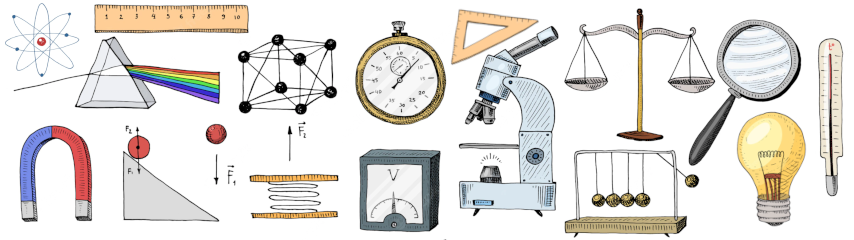
\includegraphics[width=\paperwidth]{../Unidad 2/Images/cover_bg}
\end{document}

\restoregeometry
\addtocontents{toc}{\setcounter{tocdepth}{3}}
\tableofcontents
\newpage
\chapter{}
\pagestyle{fancy}

\newpage \thispagestyle{plain}

\section{Tecnolog\'ia y transformaci\'on de la sociedad}
\boxabstract{
  Analiza cambios en la historia relativos
  a la tecnología en diversas actividades
  humanas (medición, transporte,
  industria, telecomunicaciones) para
  valorar su impacto en la vida cotidiana
  y en la transformación de la sociedad.
}
\subsection{El cambio y el tiempo}
Terminaba la d\'ecada de los setenta, yo estudiaba el \'ultimo grado de primaria
cuando conoc\'i ese novedoso invento:
la calculadora; era una de esas que hoy llamamos b\'asicas porque s\'olo hac\'ian las
operaciones de suma, resta, multiplicaci\'on
y divisi\'on, pero para m\'i y mis compañeros de grupo representaba la soluci\'on a
esas largas y laboriosas multiplicaciones
que el maestro nos dejaba de tarea.
Uno de esos d\'ias en los que mi abuelo nos visitaba, mi padre le mostr\'o el nuevo
artefacto. Nunca olvidar\'e su expresi\'on
de asombro al ver c\'omo ese pequeño objeto resolv\'ia, al instante, cualquier
operaci\'on aritm\'etica. Pero lo que m\'as me sorprendi\'o fue su pregunta:
¿C\'omo hace para resolver las operaciones? No ten\'iamos respuesta.
Responde en tu cuaderno.
?`Qu\'e inventos actuales no conocieron tus padres o tus abuelos cuando eran
niños?
?`C\'omo ha evolucionado la tecnolog\'ia en las \'ultimas d\'ecadas? ?`C\'omo ha cambiado
la vida de las personas o la sociedad a partir
de los avances tecnol\'ogicos?
?`Has notado que los niños y adolescentes usan sin mayor problema tel\'efonos
celulares, tabletas electr\'onicas y computadoras,
pero que a las personas mayores les resulta dif\'icil hacerlo? ?`A qu\'e crees que
se deba?
?`Qu\'e har\'ias para enseñar a un adulto c\'omo usar las nuevas tecnolog\'ias?

\subsubsection{El paso del tiempo}

?`C\'omo sabemos que el tiempo pasa? Las manecillas de un reloj se mueven, los
n\'umeros del reloj digital cambian, la arena de un
reloj cae. Los sucesos ocurren en el tiempo y nos muestran que el tiempo
avanza. Hay, entonces, una relaci\'on estrecha entre el
tiempo y el cambio: las cosas cambian en el tiempo y a partir del cambio
sabemos que el tiempo pasa. Este cambio es continuo e
inevitable, por medio de \'el sabemos que aunque permanezcamos est\'aticos, todo
cambia de manera constante.
Observemos a nuestro alrededor para confirmar de inmediato que las cosas
cambian: hay d\'ia y noche; el Sol sale por el este y
se oculta en el oeste; los seres vivos crecen y se desarrollan; muchos animales
se desplazan o son capaces de mover algunos de
sus \'organos. Pero tambi\'en se mueven las cosas inanimadas, como el aire y el
agua de los r\'ios, incluso el agua estancada de un
charco se evapora y forma nubes, que vuelven al suelo en forma de lluvia, nieve
o granizo; el suelo se erosiona y la rocas se
desgastan; hasta los continentes y las estrellas se mueven. Todos estos cambios
y fen\'omenos son objeto de estudio de la ciencia
en sus distintas ramas.

El ser humano se distingue de otros animales por su capacidad de modificar su
entorno, de crear artefactos y herramientas para
facilitar tareas o mejorar sus condiciones de vida. Este proceso lo ha logrado
gracias a la tecnolog\'ia, que es la aplicaci\'on de
conocimientos y habilidades en el desarrollo y creaci\'on de t\'ecnicas y objetos
para resolver necesidades o problemas pr\'acticos.
Veamos un ejemplo.

\subsubsection{Desarrollo hist\'orico de las calculadoras}
Desde que el ser humano tuvo la necesidad de hacer operaciones con n\'umeros,
como sumas, restas, multiplicaciones, ra\'ices
cuadradas, etc\'etera, ide\'o m\'etodos, algoritmos y artefactos que facilitaran o
agilizaran esas operaciones.
Dos mil años antes de nuestra era, en Mesopotamia, se invent\'o el \'abaco,
instrumento con cuentas que se deslizan en varillas.
Los antiguos matem\'aticos agrupaban o separaban las cuentas para resolver
operaciones de suma, resta, multiplicaciones y
divisiones, e incluso calculaban ra\'ices cuadradas.
En 1636 \textbf{William Oughtred (1574-1660)} invent\'o la regla de c\'alculo, que
consiste en un par de regletas deslizables con
escalas con las que se pueden hacer operaciones matem\'aticas; su uso se
populariz\'o hasta el siglo XX debido a que eran pr\'acticas
y f\'aciles de transportar.

\begin{figure}[H]
  \begin{minipage}[b]{0.5\linewidth}
    \centering
    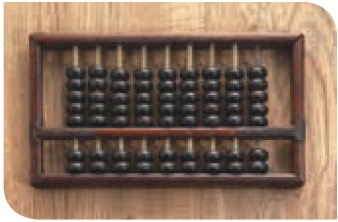
\includegraphics[width=0.7\linewidth]{abaco.jpg}
    \caption{\'Abaco}
    \label{fig:a}
  \end{minipage}%%
  \begin{minipage}[b]{0.5\linewidth}
    \centering
    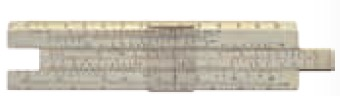
\includegraphics[width=0.7\linewidth]{regla_calculo.jpg}
    \caption{Regla de c\'alculo}
    \label{fig:b}
  \end{minipage}
  \begin{minipage}[b]{0.5\linewidth}
    \centering
    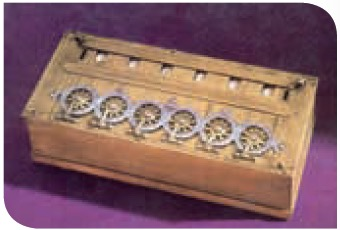
\includegraphics[width=0.7\linewidth]{pascalina.jpg}
    \caption{Pascalina}
    \label{fig:c}
  \end{minipage}%% 
  \begin{minipage}[b]{0.5\linewidth}
    \centering
    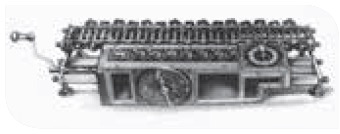
\includegraphics[width=0.7\linewidth]{maquina_Leibniz.jpg}
    \caption{M\'aquina de Leibniz}
    \label{fig:d}
  \end{minipage}
  \captionof{figure}{Evoluci\'on de instrumentos para el c\'alculo.}
  \label{fig:fig7}
\end{figure}


En el siglo XVII se inventaron las primeras calculadoras mec\'anicas, las cuales
funcionaban a base de engranes y palancas.
En 1639 el matem\'atico, f\'isico y fil\'osofo \textbf{Blaise Pascal (1623-1662)}
cre\'o la \emph{Pascalina}, instrumento para sumar y
restar que constaba de una serie de engranajes marcados con los n\'umeros del 0
al 9; cuando un engrane daba una vuelta completa,
en el siguiente engrane se sumaba una unidad.
Treinta años despu\'es el matem\'atico \textbf{Gottfried Wilhelm Leibniz
  (1646-1716)} construy\'o una calculadora similar a la
Pascalina que adem\'as de sumar y restar, multiplicaba y divid\'ia; tambi\'en usaba
engranes, los n\'umeros para los c\'alculos se
introduc\'ian por medio de botones y con una manivela se hac\'ia girar todo el
mecanismo.
Con el paso de los años este tipo de calculadoras se fueron perfeccionando, y
ya en el siglo su uso era com\'un en las tiendas
de autoservicio, incluso se fabricaron calculadoras mec\'anicas compactas que
cab\'ian en la palma de la mano, pero eran muy
costosas. En la d\'ecada de los cincuenta apareci\'o la primera calculadora de
transistores, que era del tamaño de un escritorio.
A finales de los cincuenta surgieron las primeras calculadoras b\'asicas
totalmente electr\'onicas con precios elevad\'isimos,
cerca de \$80,000 d\'olares. Fue hasta inicios de los años setenta que varias
compañ\'ias produjeron calculadoras que funcionaban
con pilas y a precios accesibles, las cuales se vendieron por todo el mundo. En
1973 aparecieron las calculadoras cient\'ificas,
que no s\'olo hac\'ian operaciones b\'asicas, sino que calculaban ra\'ices y potencias
de distintos valores, y utilizaban funciones
trigonom\'etricas y otras m\'as complejas las cuales estudiar\'as en tus cursos m\'as
avanzados de matem\'aticas. A finales del siglo XX
se incorporaron las celdas solares, por lo que ahora contamos con calculadoras
que no necesitan bater\'ias. Actualmente las
calculadoras son capaces de resolver operaciones superiores, ecuaciones y hasta
trazar gr\'aficas.
?`C\'omo se mide el tiempo?

El tiempo es una cantidad f\'isica que nos permite enmarcar el cambio y ordenar
los sucesos en secuencias, estableciendo un pasado,
un presente y un futuro.



La unidad de tiempo \emph{año} tiene su origen en el periodo que la Tierra tarda
en dar una vuelta alrededor del Sol; un \emph{d\'ia}
se refiere al tiempo en que la Tierra completa una vuelta sobre su propio eje,
y que antiguamente se determinaba como el tiempo
que transcurr\'ia entre una y otra salida del Sol. Ya desde la Antigüedad los
egipcios y sumerios dividieron el d\'ia en 24 horas,
12 para la luz diurna y 12 para la noche; la divisi\'on entre minutos y segundos
(figura 1.4) surgi\'o a partir de la necesidad
de medir los fen\'omenos celestes con m\'as precisi\'on, y fue en la Edad Media
cuando estas \'ultimas unidades se aplicaron para la
medici\'on del tiempo. Por cierto, la palabra \textbf{minuto}, tiene su origen en
la palabra latina \emph{minutus}, que significa \emph{pequeño},
y \textbf{segundo} se deriva de secundus, que significa \emph{el que va despu\'es del
  primero}, por lo que un segundo  es lo que
sigue en pequeñez a un minuto. Los subm\'ultiplos del segundo, como el
milisegundo y el microsegundo, se emplean para mediciones
muy precisas, como en fen\'omenos a nivel at\'omico.

La unidad oficial para medir el tiempo en el Sistema Internacional de Unidades
(SI) es el segundo (s\'imbolo: s), pero
cotidianamente utilizamos otras unidades, como minutos, horas, d\'ias, años,
entre otros. Observa las equivalencias:

\begin{minipage}[b]{0.5\linewidth}
  \begin{align*}
    60 \text{ segundos}    & = 1 \text{ minuto}   \\
    60 \text{ minutos}     & = 1 \text{ hora}     \\
    24 \text{ horas}       & = 1 \text{ d\'ia}    \\
    365.256 \text{ d\'ias} & = 1 \text{ año}      \\
    100 \text{ años}       & = 1 \text{ siglo}    \\
    5 \text{ años}         & = 1 \text{ lustro}   \\
    1 000 \text{ años}     & = 1 \text{ milenio}  \\
    10 \text{ años}        & = 1 \text{ d\'ecada}
  \end{align*}
\end{minipage}%
\begin{minipage}[b]{0.5\linewidth}
  Tambi\'en hay subm\'ultiplos del segundo que se basan en el sistema decimal:
  \begin{align*}
    1 \text{ segundo} & = 10   \text{ decisegundos}  \\
    1 \text{ segundo} & = 100  \text{ centisegundos} \\
    1 \text{ segundo} & = 1000 \text{ milisegundos}
  \end{align*}
\end{minipage}

\newpage
\subsubsection{Ejercicios}
Contesta lo siguiente:

\begin{enumerate}
  \item ?`Cu\'antos meses y d\'ias has vivido desde que naciste hasta hoy?
  \item ?`Cu\'antas horas hay en un siglo?
  \item ?`Cu\'antos milisegundos tiene un minuto?

  \item Elige la respuesta correcta.
        \begin{enumerate}
          \item Los seres humanos se distinguen de los animales por su capacidad de
                cambiar su entorno creando herramientas que le facilitan tareas o mejoran su
                condici\'on de vida, a esto le llamamos \dots

                \begin{hoptboxes}
                  \item F\'isica
                  \item Cultura
                  \item Meditaci\'on
                \end{hoptboxes}
          \item La herramienta m\'as antigua que conocemos, creada para facilitar los
                c\'alculos matem\'aticos es \dots

                \begin{hoptboxes}
                  \item El \'abaco
                  \item El comp\'as
                  \item La calculadora
                  \item La regla de c\'alculo
                \end{hoptboxes}
          \item Las primeras calculadoras como la inventada por Blaise Pascal en 1639
                funcionaban a base de \dots

                \begin{hoptboxes}
                  \item circuitos
                  \item engranajes
                  \item cuentas deslizables
                  \item regletas deslizables
                \end{hoptboxes}
          \item  En 1973 apareci\'o este instrumento capaz de realizar c\'alculos
                complejos como ra\'ices, potencias y  funciones trigonom\'etricas.

                \begin{hoptboxes}
                  \item \'Abaco
                  \item Calculadora b\'asica
                  \item Calculadora cient\'ifica
                  \item Regletas de c\'alculo
                \end{hoptboxes}
        \end{enumerate}

  \item Relaciona los siguientes elementos.

        \begin{minipage}{0.45\linewidth}
          \begin{enumerate}
            \item Inventor de la regla de c\'alculo.
            \item Inventor de una calculadora similar a la pascalina que pod\'ia
                  multiplicar y dividir.
            \item Este tipo de calculadora apareci\'o en los años cincuenta y fue
                  totalmente electr\'onica con precios cerca de \$80 000 d\'olares.
            \item Este tipo de calculadora resuelve operaciones con ra\'ices y
                  potencias de distintos valores. Apareci\'o en 1973.
            \item Calculadora del tamaño de un escritorio.
          \end{enumerate}
        \end{minipage}\hfill
        \begin{minipage}{0.4\linewidth}
          \begin{itemize}
            \item[\Huge$\square$] Calculadora b\'asica \vspace{0.5cm}
            \item[\Huge$\square$] Gottfried Wilhelm Leibnitz  \vspace{0.5cm}
            \item[\Huge$\square$] William Oughtred	  \vspace{0.5cm}
            \item[\Huge$\square$] Calculadora de transistores    \vspace{0.5cm}
            \item[\Huge$\square$] Calculadora cient\'ifica   \vspace{0.5cm}
          \end{itemize}

        \end{minipage}

  \item Ordena los nombres de los creadores de instrumentos de c\'alculo,
        del m\'as antiguo al m\'as reciente.

        \begin{itemize}
          \item[\rule{1cm}{0.2pt}] Gottfried Leibniz
          \item[\rule{1cm}{0.2pt}] William Oughtred
          \item[\rule{1cm}{0.2pt}] Blaise Pascal
        \end{itemize}
\end{enumerate}

\newpage \thispagestyle{plain}
\section{ Velocidad y aceleraci\'on}
\boxabstract{Comprende los conceptos de velocidad y aceleración.}
\subsection{El movimiento de los objetos}
Para describir el movimiento de un objeto, primero tenemos que describir su posición;
es decir, en dónde está en cualquier momento en particular. Para ello, necesitamos primero
establecer cuál es el marco de referencia del sistema que vamos a estudiar. Un marco o
sistema de referencia consta de un origen, o sea, el punto desde el que se consideran
las medidas de distancia, dirección, rapidez, etcétera, y de un sistema coordenado
que permite determinar la escala de las medidas.

Algunos ejemplos de marcos de referencia:
\begin{itemize}
  \item La recta numérica
  \item El plano cartesiano
  \item El Sistema Solar con origen en el Sol
  \item Sistema esférico terrestre con origen en el centro de la Tierra.
\end{itemize}


Observen el siguiente plano cartesiano (figura \ref{fig:plano01})  y respondan.
El largo de cada cuadrado de la retícula representa una unidad.
\begin{figure}[H]
  \centering
  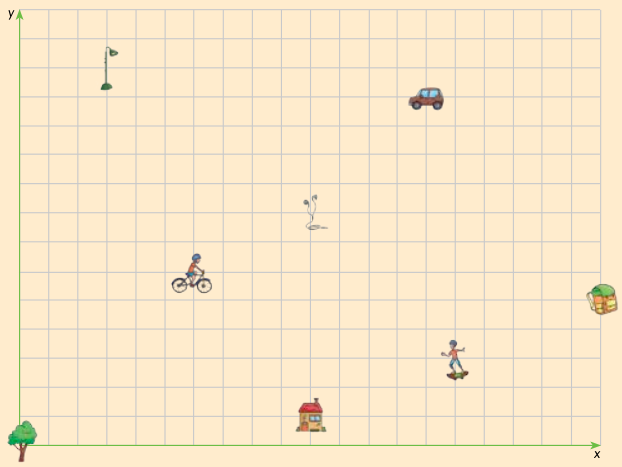
\includegraphics[width=0.8\textwidth]{plano01.png}
  \captionof{figure}{}
  \label{fig:plano01}
\end{figure}
\begin{enumerate}
  \item Considerando la posición del árbol como origen del sistema de referencia indiquen la posición
        de los audífonos, el carro y la mochila. Tomen el centro de cada figura para ubicar su posición
        \begin{align*}
          \text{audifonos} & = ( \quad, \quad ) \\
          \text{carro}     & = ( \quad, \quad ) \\
          \text{mochila}   & = ( \quad, \quad )
        \end{align*}
  \item Consideren ahora como origen la posición del farol y señala la posición del joven con patineta,
        la bicicleta y la casa.
        \begin{align*}
          \text{patineta}  & = ( \quad, \quad ) \\
          \text{bicicleta} & = ( \quad, \quad ) \\
          \text{casa}      & = ( \quad, \quad )
        \end{align*}
  \item ¿Qué objeto se encuentra en la coordenada $(0, 7)$ considerando la casa como origen del sistema de
        referencia?
  \item Si el origen es el joven con patineta, ¿qué objeto está en la coordenada $(5, 2)$? ¿Y en la
        coordenada $(-5, -2)$?
  \item ¿Un objeto puede tener dos o más coordenadas distintas? ¿Por qué?


\end{enumerate}


\subsubsection{Trayectoria, desplazamiento y distancia recorrida}
La
trayectoria es la línea imaginaria que une todos los
puntos por los que pasó un
objeto. ¿Cuál es la relación entre el trazo que dejaron
las canicas y la trayectoria que siguieron en su movimiento?

Otro concepto importante en la descripción del movimiento es
la distancia, con la cual estás familiarizado desde la primaria, ya
que has medido distancias, como la longitud de una recta, los la
dos de figuras geométricas, tu estatura, etcétera, y para ello has
usado una regla, un flexómetro o una cinta métrica.
¿Qué es entonces la distancia? La distancia es la medida de la lon
gitud que separa dos puntos.


\begin{figure}[H]
  \centering
  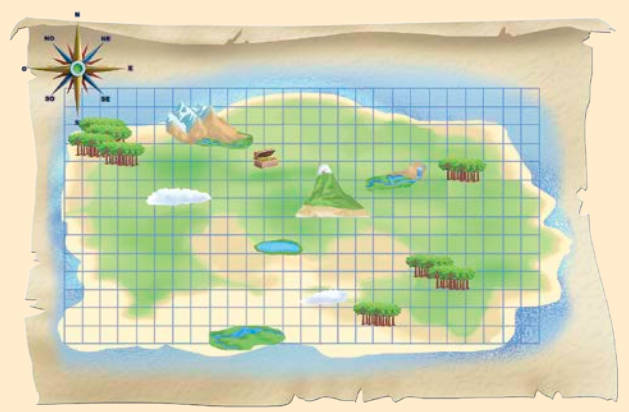
\includegraphics[width=0.8\textwidth]{plano02.png}
  \captionof{figure}{Mapa coordenado del tesoro}
  \label{fig:plano02}
\end{figure}
Supón que el siguiente mapa es de una isla deshabitada y tienes que seguir las indicaciones
para localizar el tesoro.
\begin{enumerate}
  \item Traza los ejes del plano cartesiano y en ellos indica los puntos cardinales.
        Considera la esquina inferior izquierda como el punto $(0, 0)$.
        \emph{Tu recorrido inicia en la playa, en la coordenada $(0, 0)$.
          Camina 5 pasos hacia el este, 6 hacia el norte, 15 otra vez hacia el este, 2 hacia el sur,
          6 hacia el oeste, 4 hacia el sur, 10 hacia el este, 12 al norte, 13 hacia el oeste y
          si avanzas 2 más hacia el sur, encontrarás el tesoro.} ¿Lo encontraste?
        (Un paso representa la distancia del lado de cada cuadro de la retícula).
  \item ¿Cuál es el sistema de referencia?
  \item ¿Cuál es el origen del sistema de referencia?
  \item Traza en el mapa la trayectoria del movimiento.
  \item Menciona el punto exacto en que se encuentra el tesoro usando coordenadas.
  \item ¿Cuántos pasos recorriste para encontrar el tesoro?
  \item Anota en tu cuaderno otra serie de instrucciones para llegar al tesoro y calcula cuántos
        pasos se recorren esta vez.
  \item Si hubieras caminado en línea recta desde el punto de inicio hasta el lugar del tesoro,
        ¿cuántos pasos habrías dado? ¿En qué dirección habrías caminado?
\end{enumerate}

\subsubsection{El cambio de la posición}
Si un objeto se mueve en relación a un marco de referencia, entonces la posición del objeto
cambia. A este cambio en la posición se le conoce como desplazamiento. La palabra desplazamiento
implica que un objeto se movió, o se desplazó.

El desplazamiento ($\Delta x$) se define como el cambio en la posición de un objeto.
Se puede definir de
manera matemática con la siguiente ecuación:
\[\Delta x = x_f - x_i\]
donde:

$xf$ se refiere al valor de la posición final.\\
$x_i$ se refiere al valor de la posición inicial.\\
$\Delta x$ es el símbolo que se usa para representar el desplazamiento.\\

\subsubsection{Ejercicios}
\begin{enumerate}
  \item Para cubrir su ruta por la ciudad un autobús se desplaza 5 km hacia el oeste, gira hacia la izquierda y recorre 3 km, da vuelta hacia el este y avanza 10 km, luego recorre 5 km al norte, de nuevo viaja hacia el este 5 km y finalmente se desplaza 2 km hacia el sur. ¿Qué distancia recorrió y cuánto mide su desplazamiento?
  \item Traza el movimiento de un objeto cuyo desplazamiento coincide con su trayectoria. ¿Qué forma tiene la trayectoria?
  \item Traza la trayectoria de un objeto cuya distancia recorrida sea distinta de cero,
        pero que su desplazamiento sea cero.
  \item Si un objeto se encuentra en la coordenada $(4, 5)$ de un plano cartesiano y dos
        segundos después su posición es $(7, 5)$, ¿qué distancia recorrió en ese tiempo?
        Describe el desplazamiento correspondiente; las unidades están en metros.
\end{enumerate}

\newpage
\subsection{La velocidad y la rapidez}
\subsubsection{Rapidez}
La rapidez es un concepto que involucra distancia (sin importar la dirección o sentido) y tiempo,
y se define como el cociente entre la distancia recorrida $d$ y el tiempo $t$ para recorrerla,
que matemáticamente se expresa como:
\begin{equation}
  r=\frac{d}{t}
\end{equation}
donde:\\
$r$ es la rapidez del movimiento (medida en m/s)\\
$d$ es la distancia recorrida (medida en m),\\
$t$ es el tiempo de recorrido (medida en s)


\subsubsection{Ejemplos}

\begin{figure}[H]
  \centering
  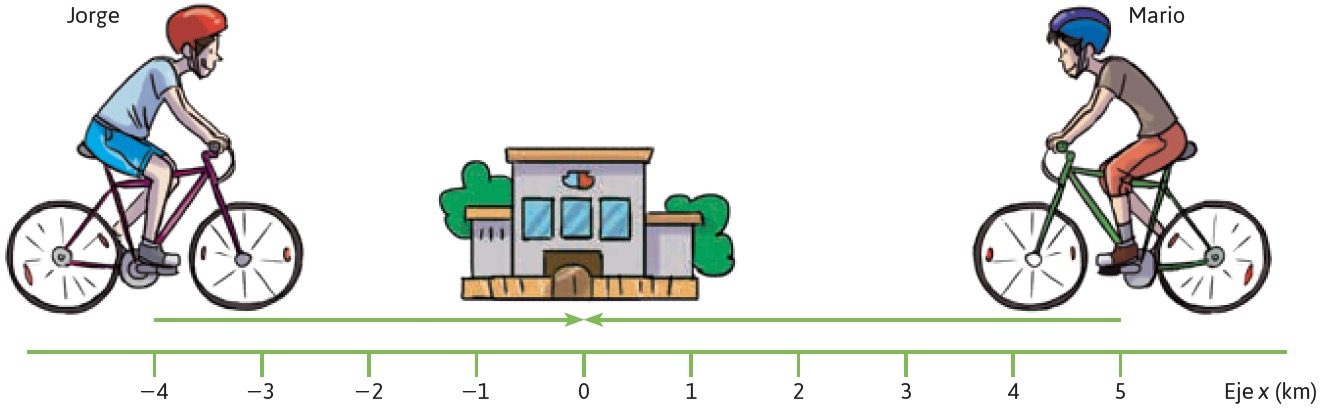
\includegraphics[width=0.8\textwidth]{mario_jorge.jpg}
  \captionof{figure}{Mapa coordenado del tesoro}
  \label{fig:mario_jorge}
\end{figure}
\begin{enumerate}

  \item Mario y Jorge van a la escuela en bicicleta. Mario vive a 5 kilómetros de distancia al este
        de la escuela, y Jorge, a 4 kilómetros, pero al oeste (tal y como se muestra en la
        figura \ref{fig:mario_jorge}).
        \begin{enumerate}
          \item Si ambos salen de sus casas a las 6:40
                y llegan a la escuela al mismo tiempo a las 6:55, calcula la rapidez de
                Mario y Jorge a partir de la definición anterior.
                (Consideren que las unidades de tiempo están en horas.)
                \begin{align*}
                  r_{\text{M}} & =\frac{d}{t}=\frac{\quad \text{ km}}{\quad \text{ h}} \\
                  r_{\text{J}} & =\frac{d}{t}=\frac{\quad \text{ km}}{\quad \text{ h}}
                \end{align*}

          \item ¿Cómo son los cocientes de ambas operaciones?
          \item ¿Quién fue el más rápido?
          \item Calculen la rapidez para el inciso b de la actividad anterior.
          \item Cuando salieron de clase, fueron a la casa de Mario a hacer su proyecto
                de Ciencias. Jorge llegó en 15 minutos y Mario en 20 minutos.
                ¿Quién fue el más rápido? ¿Por qué?
        \end{enumerate}

        \begin{figure}[H]
          \centering
          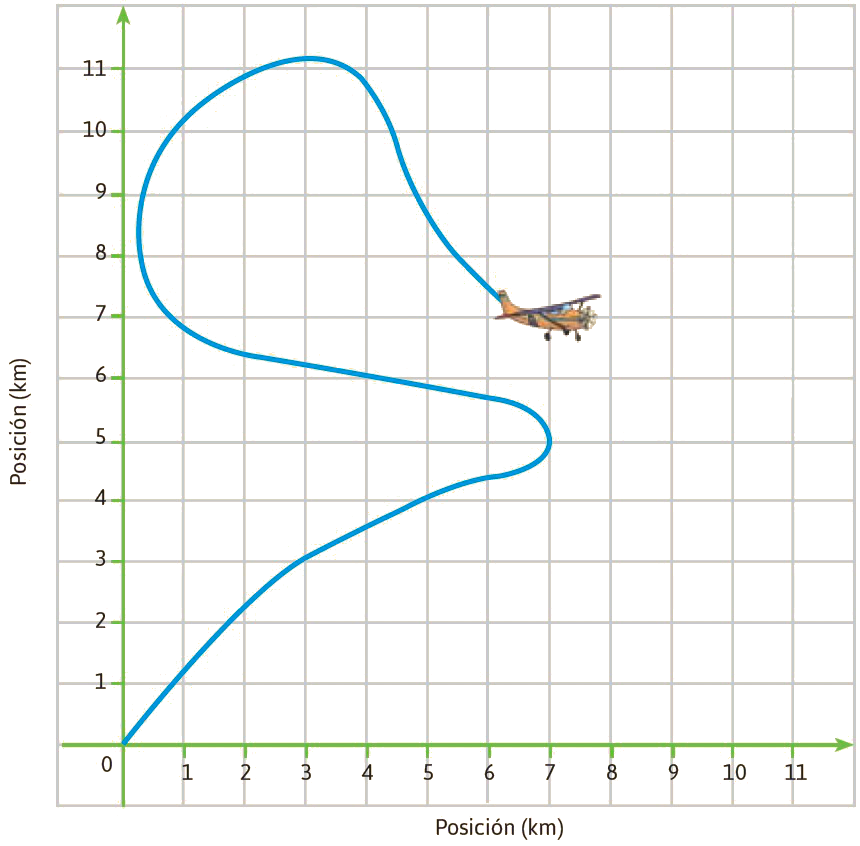
\includegraphics[width=0.8\textwidth]{avioneta01.png}
          \captionof{figure}{Mapa coordenado del tesoro}
          \label{fig:avioneta01}
        \end{figure}
  \item En el plano cartesiano de la figura \ref{fig:avioneta01} se muestra el movimiento
        de una avioneta. Obsérvala, realiza lo que se pide y responde.
        \begin{enumerate}
          \item Midan la distancia recorrida.
          \item Señalen en el plano el desplazamiento. ¿Cuál es su longitud?
          \item Si la avioneta realizó su recorrido en 15 min, ¿cuál fue su rapidez media?
          \item ¿Cuál fue la velocidad media de la avioneta?
          \item Cómo determinaron la distancia que recorrió la avioneta?
          \item ¿Cómo obtuvieron el desplazamiento?
          \item ¿La rapidez y la velocidad de la avioneta fueron iguales o distintas? ¿Por qué?
        \end{enumerate}
\end{enumerate}

\newpage
\subsubsection{Velocidad}
La velocidad es la magnitud que relaciona el cambio en la posición de un objeto
(desplazamiento) dividido entre el tiempo, y se expresa de la siguiente manera:
\begin{equation}
  v=\frac{\Delta x}{t}
\end{equation}
donde:\\
$v$ es la velocidad del movimiento (medida en m/s)\\
$d$ es la distancia recorrida (medida en m),\\
$t$ es el tiempo de recorrido (medida en s)

La velocidad es, por tanto, el cociente del cambio de posición de un objeto y el tiempo que tarda
en recorrerlo, por lo que incluye dirección y sentido. Así decimos que la rapidez de Mario es de
20 km/h y su velocidad, de -20 km/h, o de 20 km/h en dirección oeste.

Observa que las unidades de la rapidez y de la velocidad son las mismas: unidades de distancia
o posición entre unidades de tiempo. En el si se emplean metros por segundo, m/s, pero
también se usan múltiplos o submúltiplos de ellas; por ejemplo, en las carreteras seguramente
has visto que la rapidez se indica en kilómetros por hora km/h y en algunos países de habla
inglesa se señalen millas por hora, mi/h; la rapidez de la luz es de 300,000 km/s;
la del sonido en el aire, de 343 m/s y la de un caracol, 1.3 cm/s. ¿Por qué piensas que
se expresan en esas unidades?

Cabe mencionar que la rapidez y la velocidad de los ejemplos anteriores corresponden a la
\textbf{rapidez y velocidad media o promedio}, ya que sólo se consideran tiempos y distancias totales
para la rapidez, o las posiciones y tiempos iniciales y finales para la velocidad.

En el movimiento en un plano o en el espacio, la rapidez se obtiene determinando la distancia
que recorre el objeto en movimiento y se divide entre el tiempo; para la velocidad hay que
considerar el desplazamiento que incluye la dirección y el sentido del movimiento.

Es poco probable que la avioneta de la actividad anterior siempre se moviera con la misma
rapidez: inició en reposo, después la aumentó al despegar y disminuyó al aterrizar.
En este caso, la rapidez que calculaste fue la rapidez media o promedio. Conocer la rapidez
de un objeto en cada momento de su trayectoria es más complicado, y se conoce como \textbf{rapidez
  instantánea}, ya que se refiere a un instante preciso.

Por ejemplo, si un autobús se detiene porque en su trayecto encuentra un semáforo en rojo,
en ese momento su rapidez instantánea es cero. De igual manera, a la velocidad de un objeto
en un momento preciso se conoce como \textbf{velocidad instantánea}.

\begin{figure}[H]
  \centering
  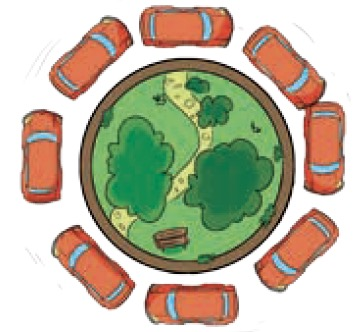
\includegraphics[width=0.4\textwidth]{glorieta.jpg}
  \captionof{figure}{En el movimiento circular un objeto cambia constantemente de velocidad.}
  \label{fig:glorieta}
\end{figure}

Observa la figura \ref{fig:glorieta}. Si el automóvil se mueve alrededor de la glorieta
con rapidez constante, ¿su velocidad también es constante? Un objeto puede moverse siempre
con la misma rapidez instantánea, pero su velocidad instantánea puede cambiar; por ejemplo,
un objeto que se mueve en círculos puede siempre tener la misma rapidez, pero como su dirección
cambia en cada momento, su velocidad instantánea no es la misma.

\begin{figure}[H]
  \centering
  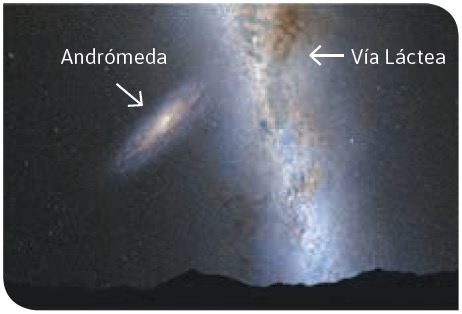
\includegraphics[width=0.4\textwidth]{galax.jpg}
  \captionof{figure}{Andrómeda y la Vía Láctea vistas desde la Tierra. Si continúan moviéndose con la misma rapidez, colisionarán en 5,000 millones de años.}
  \label{fig:galax}
\end{figure}

Al iniciar la secuencia estudiamos que en el Universo todo está en continuo cambio y movimiento,
y que el movimiento depende del marco de referencia desde el que se observa. Como sabemos,
la Tierra gira sobre su propio eje y completa una vuelta en 24 horas, pero además, nuestro
planeta se mueve alrededor del Sol dando una vuelta cada año. Asimismo, el Sol se mueve alrededor
de la galaxia con una rapidez de 792,000 km/h jalando con él a todo el Sistema Solar, y nuestra
galaxia, la Vía Láctea, se acerca a su vecina, la galaxia de Andrómeda con una rapidez de
468,000 km/h, (figura \ref{fig:galax}). Y no sólo eso, las galaxias se mueven alejándose a grandes
velocidades. Una vez más cabe la pregunta: ¿nos movemos?, ¿con qué rapidez?

\subsubsection{Ejercicios}
\begin{enumerate}
  \item Usain Bolt, atleta jamaiquino considerado el ser humano más rápido del mundo,
        posee los récords mundial y olímpico en carreras de 100 y 200 metros planos. En el
        campeonato mundial de Berlín corrió los 100 metros planos en 9.58 segundos, y en los
        juegos olímpicos de Londres en 2012, en 9.63 segundos. ¿En cuál de las dos competencias
        fue más rápido? Justifica tu respuesta.
  \item En el ciclismo, el llamado récord de la hora consiste en que el ciclista trate de
        recorrer la mayor distancia posible en ese tiempo. En enero de 2016, la ciclista australiana
        Bridie O'Donell recorrió 46882 m y en febrero del mismo año la estadounidense Evalyn Stevens,
        47,980 m también en una hora. ¿Quién fue la más rápida? Explica.
  \item En una zona terrestre representada en un mapa mediante un plano cartesiano donde
        la dirección del eje de las x coincide con la dirección este-oeste, y la del eje de las y,
        con la dirección norte-sur, a las 10:39 hrs un camión se encontraba en la coordenada
        $(20, 20)$, y a las 11:45 hrs en la posición $(60, 60)$. Considera que las unidades están
        en kilómetros y realiza lo siguiente.
        \begin{enumerate}
          \item En tu cuaderno traza un plano cartesiano y, con una escala adecuada, ubica la
                posición inicial y final del camión.
          \item Señala el desplazamiento y estima la distancia recorrida a partir de la escala.
          \item Determina la rapidez con la que el camión se movió desde la posición inicial
                hasta la posición final.
          \item Describe la velocidad del camión utilizando los puntos cardinales.
        \end{enumerate}
  \item Si la circunferencia de la Tierra es de 40,075 km, ¿con qué rapidez se mueve una persona
        que se encuentra sobre el ecuador?
  \item Nuestro planeta se mueve en una órbita casi circular de aproximadamente 150,000,000 km
        alrededor del Sol. ¿Cuál es su rapidez de traslación?
  \item Un avión supersónico puede volar con una rapidez de 1,225 km/h. ¿Qué distancia recorrería
        con esa rapidez en 12.5 h?
  \item Una nave espacial se desplaza con una rapidez de 40,300 km/h. ¿Cuánto tiempo tardaría en
        llegar a la estrella Próxima Centaury que está a una distancia aproximada de 9 461 000 000 000 km?
  \item Próxima Centaury es la estrella más cercana a nosotros después del Sol.
        Si la humanidad se aventurara en viajar a ella, ¿cuántas generaciones tendrían
        que pasar para llegar? Considera 70 años para cada generación.
  \item La rapidez máxima posible en el Universo es la velocidad de la luz, que es cercana a
        los 300,000 km/s. Si un rayo de luz del Sol tarda casi 8 minutos con 19 segundos
        en llegar a nuestro planeta, ¿cuál es la distancia de la Tierra al Sol?
  \item En sus últimas vacaciones, Raúl y su familia decidieron hacer un viaje en carretera. Primero fueron a la ciudad de Querétaro. El viaje fue de 300 km y lo completaron en 3 horas. Posteriormente viajaron a Monterrey, que se encuentra a 700 km, y les tomó 5 horas llegar ahí.
        \begin{enumerate}
          \item ¿Cuál es el valor de su velocidad media en la primera etapa de su viaje?
          \item ¿Cuál es el valor de su velocidad media en la segunda etapa?
          \item ¿Cuál es el valor de su velocidad media en todo el viaje?
        \end{enumerate}
  \item Indica si las siguientes afirmaciones son Verdaderas o Falsas:
        \begin{enumerate}
          \item La velocidad y la rapidez se miden en unidades distintas.\\
                \begin{hoptboxes}
                  \item Verdadero
                  \item Falso
                \end{hoptboxes}
          \item No es lo mismo desplazamiento que trayectoria.\\
                \begin{hoptboxes}
                  \item Verdadero
                  \item Falso
                \end{hoptboxes}
          \item La rapidez tiene dirección y sentido.\\
                \begin{hoptboxes}
                  \item Verdadero
                  \item Falso
                \end{hoptboxes}
          \item La velocidad es el cociente del cambio de posición de un objeto y el tiempo que tarda en recorrerlo.\\
                \begin{hoptboxes}
                  \item Verdadero
                  \item Falso
                \end{hoptboxes}
        \end{enumerate}

\end{enumerate}

\newpage
\subsection{Gr\'aficas que representan la velocidad (desplazamiento vs. tiempo)}
En la siguiente tabla \ref{tab:caballos_tabla} se registran los datos de desplazamiento y
tiempo de Relámpago y Arabela,
dos caballos de carreras, durante una competencia en un tramo recto.
Los desplazamientos se miden desde el lugar de salida que corresponde al origen.
\begin{figure}[H]
  \centering
  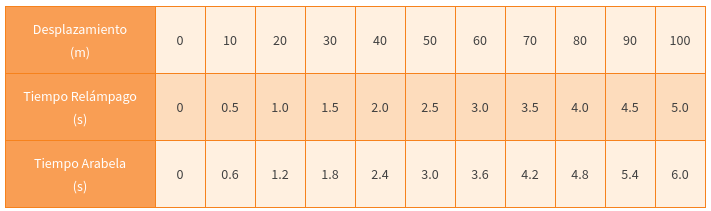
\includegraphics[width=0.8\textwidth]{caballos_tabla.png}
  \captionof{table}{Datos de desplazamiento y tiempo de Relámpago y Arabela.}
  \label{tab:caballos_tabla}
\end{figure}


\begin{minipage}[t]{0.5\linewidth}
  \begin{figure}[H]
    \centering
    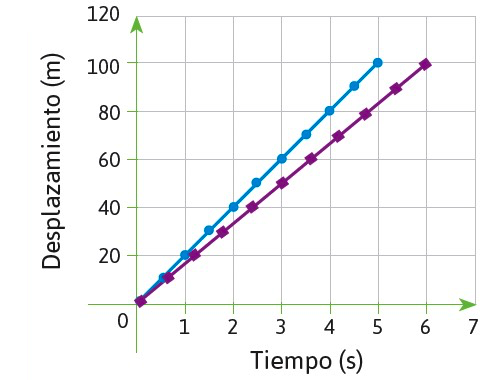
\includegraphics[width=\linewidth]{caballos_fig.jpg}
    \captionof{table}{Gr\'afica de desplazamiento y tiempo de Relámpago y Arabela.}
    \label{fig:caballos_fig}
  \end{figure}
\end{minipage}
\begin{minipage}[t]{0.5\linewidth}
  La gráfica \ref{fig:caballos_fig} muestra los datos de la tabla. Analízala  responde en tu cuaderno.
  \begin{enumerate}
    \item ¿Cuál gráfica representa el movimiento de Relámpago?, y ¿cuál el de Arabela?
          ¿Cómo lo supieron?\\[1cm]
    \item Si la pista de carreras mide 100 m de largo, ¿cuál de los dos caballos fue el ganador?
          ¿Cómo lo saben?\\[1cm]
    \item Explica con tus propias palabras qu\'e significa que las gr\'aficas que relacionan
          desplazamiento y tiempo en la carrera de Relámpago y Arabela sean líneas rectas.\\[1cm]
  \end{enumerate}
\end{minipage}

\subsubsection{Gráficas de rapidez, relación distancia-tiempo}

\begin{minipage}[t]{0.65\linewidth}
  En el siglo XVII, \textbf{René Descartes (1596-1650)} (figura \ref{fig:descartes}) ideó los
  \emph{planos cartesianos}, que ya utilizamos en la primera lección de esta secuencia, los cuales
  facilitan el estudio de las gráficas.\\

  Las gráficas son valiosas herramientas porque permiten representar las relaciones entre dos
  grupos de datos, como los de desplazamiento y tiempo del ejemplo anterior. En el eje horizontal,
  o de las $x$, ubicamos los valores del tiempo, y en el eje vertical, o de las $y$, los datos de
  desplazamiento. Así, a cada par ordenado de posición y tiempo de cada caballo le corresponde
  un punto en la gráfica.\\

  Observa que en la tabla \ref{tab:caballos_tabla} los datos de desplazamiento de Relámpago y Arabela aumentan de manera
  proporcional a los del tiempo; si el tiempo aumenta al doble, de 0.5 s a 1.0 s, la distancia
  con respecto a la línea de salida que recorre Relámpago también aumenta al doble, de 10 m a 20 m;
  si el tiempo aumenta al triple, de 0.5 s a 1.5 s, la distancia también se incrementa al triple,
  de 10 m a 30 m, y, como has visto en tu curso de Matemáticas 1, esto significa que se trata de
  una relación de proporcionalidad directa.

  La gráfica de la relación entre desplazamiento y tiempo de cada caballo se representa por una
  línea recta que pasa por el origen, lo cual también significa que se trata de una relación de
  proporcionalidad directa.
\end{minipage}\hfill
\begin{minipage}[t]{0.3\linewidth}
  \begin{figure}[H]
    \centering
    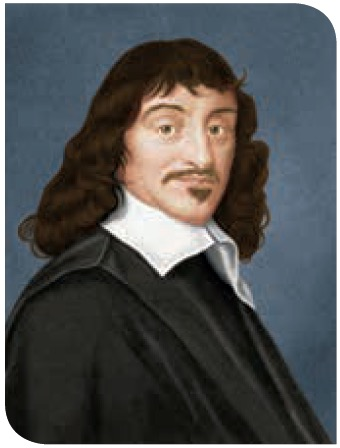
\includegraphics[width=\linewidth]{descartes.jpg}
    \captionof{figure}{René Descartes, destacado matemático, físico y filósofo francés, entre
      cuyos principales aportes está haber relacionado la geometría con el álgebra.}
    \label{fig:descartes}
  \end{figure}
\end{minipage}

Verifica que, si multiplicas la constante de proporcionalidad por los valores de tiempo,
obtienes los de desplazamiento. ¿Esta relación se cumple para cualquier intervalo? Compruébalo.

Observa que la constante de proporcionalidad corresponde a la velocidad. Si la velocidad
de un móvil no cambia en todo su recorrido, se dice que se mueve con velocidad constante
y su representación gráfica es una línea recta. Existe una relación entre la inclinación
y la velocidad: a mayor inclinación, mayor velocidad y a menor inclinación, menor velocidad.
¿A quién corresponde la gráfica más inclinada, a Relámpago o a Arabela?

Hasta el momento hemos considerado desplazamiento de los caballos y tiempo y los hemos
relacionado con la velocidad, pero también podemos tener en cuenta sólo valores de distancia
y tiempo que, como sabes, se relacionan con la rapidez.

Considera la siguiente situación. Un objeto se mueve en línea recta como se indica en la tabla
\ref{fig:recta01}.
\begin{figure}[H]
  \centering
  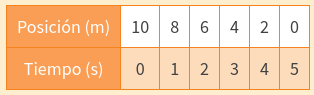
\includegraphics[width=0.5\linewidth]{recta01.png}
  \captionof{table}{}
  \label{fig:recta01}
\end{figure}


\subsection{La aceleraci\'on como cambio de la velocidad}

\newpage \thispagestyle{plain}
\section{ Movimiento ondulatorio}
\subsection{Ondas para ver}
\newpage \thispagestyle{plain}
\section{ Concepto de fuerza}
\boxabstract{
  \begin{itemize}
    \item Describe, representa y experimenta
          la fuerza como la interacción entre
          objetos y reconoce distintos tipos de
          fuerza.
    \item Identifica y describe la presencia de
          fuerzas en interacciones cotidianas
          (fricción, flotación, fuerzas en
          equilibrio).
  \end{itemize}
}


\subsection{La fuerza como interacci\'on entre los objetos}
\begin{boxK}
  \begin{center}\textbf{\color{colorrds}Inicio}\end{center}
  Levitar, es decir, elevarse en el aire, ha sido uno de los actos que más han fascinado
  al ser humano, desde aquellas leyendas de alfombras voladoras en las historias de
  \emph{Las mil y una noches} hasta los trucos de los \emph{magos} que aún despiertan la
  admiración de cientos de espectadores.
  \begin{enumerate}
    \item ¿Realmente es posible la levitación?
    \item ¿Qué fuerzas se deben vencer para levantar un objeto?
    \item ¿Por qué caen las cosas?
    \item ¿Cómo harías levitar un objeto? Propón un truco y preséntalo ante el grupo;
          después explica cómo logra levitar.
  \end{enumerate}
\end{boxK}
\subsubsection{¿Qué es la fuerza?}
La palabra \emph{fuerza} se utiliza en distintas situaciones cotidianas; por ejemplo,
Gerardo dice que debe asear la casa \emph{a fuerza}, porque prefería ver el futbol;
Angélica afirma que ella y Enrique están unidos por la \emph{fuerza}del amor, pero
Jimena opina que es más bien por la \emph{fuerza} de la costumbre, y muchos dicen que doña Agustina
es atemorizante porque tiene un carácter \emph{fuerte}. Esta palabra también permite describir
lo que se hace en relación con los objetos: a quien puede cargar bultos de 100 kg merece
que lo llamemos \emph{fuerte}, y logramos romper algo si lo golpeamos, empujamos, jalamos o
lanzamos con la fuerza suficiente. \\

En física este término se utiliza de un modo especial;
decimos, por ejemplo, que para mover un objeto pesado, como un auto, hay que aplicar mucha
fuerza; en cambio, para mover un objeto ligero, por ejemplo un globo, afirmamos que no se
necesita mucha fuerza. Igualmente decimos que para aplastar una lata se necesita de tanta
fuerza que sólo una persona muy fuerte puede hacerlo; en cambio, para deformar un poco de
plastilina no se requiere gran fuerza.\\

En la secuencia 1 vimos que las cosas cambian; sin embargo, no lo hacen por sí solas,
sino por su interacción con otras. Así, una persona empuja su auto descompuesto para
moverlo, el agua de una olla puesta al fuego hierve, las ramas de los árboles se mueven
con el viento, un globo inflado con helio se eleva, un florero cae al suelo y se rompe.\\

¿Se te ocurren otros ejemplos?\\
¿Es necesario que los objetos estén en contacto para que interactúen?\\

\begin{minipage}[t]{0.35\textwidth}
  \begin{figure}[H]
    \centering
    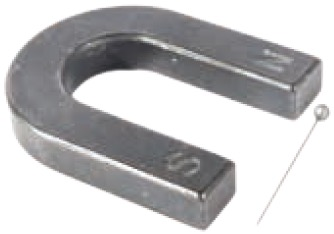
\includegraphics[width=\linewidth]{f_magnetica}
    \captionof{figure}{La fuerza magnética actúa a distancia.}
    \label{fig:f_magnetica}
  \end{figure}
  \begin{figure}[H]
    \centering
    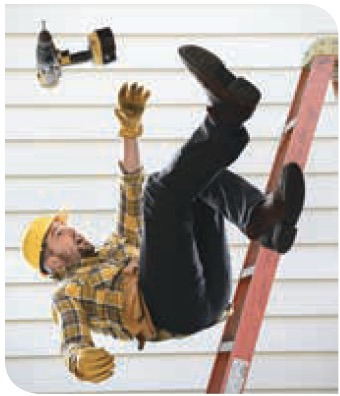
\includegraphics[width=\linewidth]{f_gravitacional}
    \captionof{figure}{Los cuerpos caen debido a la fuerza de gravedad que actúa a distancia.}
    \label{fig:f_gravitacional}
  \end{figure}
\end{minipage}\hfill
\begin{minipage}[t]{0.55\textwidth}

  En física se distinguen dos tipos de interacciones: por \textbf{contacto} y \textbf{a distancia}.
  Las primeras, también llamadas \textbf{mecánicas}, ocurren si los cuerpos que interactúan entran
  en contacto físico: cuando se jala, arrastra, empuja, sopla, etcétera, un cuerpo.
  En las interacciones a distancia no es necesario que los objetos involucrados estén en contacto.
  Todos los objetos interactúan entre sí, es decir, se afectan mutuamente: si jalas algo,
  sientes un \emph{jalón} del objeto; cuando dos autos chocan, ambos cambian su estado de movimiento
  y su forma: se detienen o cambian su velocidad, la lámina se comprime, el parabrisas se estrella,
  etcétera.\\

  Una \textbf{fuerza} es una interacción entre dos o más objetos y se caracteriza por su capacidad de
  cambiar la forma, el tamaño o el movimiento del objeto sobre el cual se aplica; por ejemplo,
  cuando comprimes una pelota puedes modificar su forma; si aprietas suficiente, quizá logres
  desinflarla y cambiar su tamaño, y con un golpe podrás modificar su movimiento.

  Es evidente quién o qué ocasiona las interacciones por contacto, en cambio, en las interacciones
  a distancia, si no contamos con los conocimientos previos al respecto, no siempre es fácil
  saber quién o qué genera el cambio en los objetos. Así, un alfiler se mueve si le acercamos
  un imán; este es un ejemplo de interacción magnética a distancia (figura \ref{fig:f_magnetica}),
  mientras que
  el papel y el globo de la actividad anterior mostraron un caso de interacción electrostática
  a distancia (en la unidad 2 estudiaremos más sobre los fenómenos relacionados con la electricidad
  y el magnetismo).

  Seguramente has experimentado que al soltar un objeto desde cierta altura éste cae al suelo.
  ¿Con qué interactúa el objeto para provocar su movimiento de caída?
\end{minipage}\\

Si el estado de movimiento
del objeto se modifica al caer, entonces hay una fuerza actuante. ¿Esa fuerza es de contacto o
a distancia? ¿Por qué?
La fuerza que hace caer a los objetos es la misma que mantiene a la Tierra y a los planetas
girando alrededor del Sol y recibe el nombre de \textbf{fuerza de gravedad}, que estudiarás más
adelante.
El peso de los objetos es la medida de esa fuerza.
\newpage

\subsubsection{La medición de la fuerza}


¿Cómo podemos medir una fuerza? ¿De qué manera sabemos cuándo se ha aplicado una fuerza y su
magnitud? Medir la magnitud de una interacción por su efecto en los objetos indica qué tan
grande o pequeña es la fuerza aplicada. En otras palabras, la magnitud de una fuerza está
estrechamente relacionada con los cambios (en el movimiento o la forma) que provoca en los
cuerpos sobre los que se ejerce: el cambio es el efecto de aplicar una fuerza. Esta propiedad
se aprovecha por los dinamómetros. Por ejemplo, algunos utilizan resortes que se estiran o
comprimen a la aplicar una fuerza. La magnitud de la deformación indica la fuerza aplicada.

En este momento cabe aclarar que \textbf{masa} y \textbf{peso} no son lo mismo, la masa es la
cantidad de materia
que tiene un objeto. Pero existe una relación muy estrecha entre masa y peso: un objeto con más
masa es más pesado que uno con menos masa. La masa y el peso son cantidades proporcionales y
por eso en la vida cotidiana utilizamos estos conceptos de manera indistinta. En estricto sentido,
un dinamómetro no mide la masa, sino el peso de los objetos, es decir, la magnitud de la fuerza.
Las unidades de fuerza son los \textbf{newtons (N)} (que estudiaremos más adelante).
La fuerza que ejerce
una masa de 1 kilogramo se conoce como kilogramo-fuerza y equivale a 9.8 N.

%\newpage
\subsubsection{Fuerza de flotación}

\begin{minipage}[t]{0.3\textwidth}
  \begin{figure}[H]
    \centering
    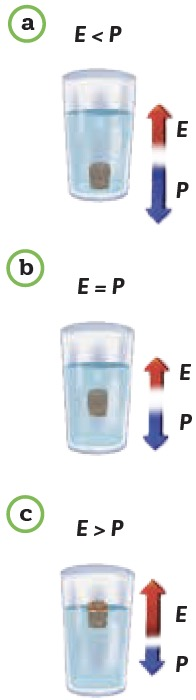
\includegraphics[width=0.6\linewidth]{vaso_arquimedes.jpg}
    \captionof{figure}{Cuerpo sumergido en un fluido. $E$ es la fuerza de empuje y
      $P$ representa su peso.}
    \label{fig:vaso_arquimedes}
  \end{figure}
\end{minipage}\hfill
\begin{minipage}[t]{0.7\textwidth}
  ¿Alguna vez has tratado de sumergir una pelota en una tina con agua? ¿Se sumerge fácilmente una
  piedra en un estanque? ¿Dónde desciende más rápido una piedra, en el aire o en el agua?\\

  Todos los objetos sumergidos en algún fluido experimentan una fuerza ascendente. Esta fuerza es
  la causa de que algunos objetos floten, por lo que se conoce como fuerza de flotación.\\

  En el siglo III a. n. e. \textbf{Arquímedes de Siracusa (287 a. n. e.-212 a. n. e.)}, un matemático griego,
  descubrió que \emph{todo cuerpo sumergido en un fluido experimenta una fuerza de empuje vertical
    igual al peso del volumen del fluido desalojado por el objeto}, a esta afirmación se le conoce
  como principio de Arquímedes.\\

  Por tanto, en todo cuerpo sumergido en un fluido, actúan dos fuerzas principalmente: su propio
  peso y la fuerza de empuje, y dependiendo de la magnitud de éstas se presentan 3 situaciones:
  si el peso es mayor que el empuje, el cuerpo se hunde (figura \ref{fig:vaso_arquimedes}a); si el peso y el empuje son
  iguales, el cuerpo no se hunde ni emerge (figura \ref{fig:vaso_arquimedes}b); si el empuje es mayor que el peso, el
  objeto flota (figura \ref{fig:vaso_arquimedes}c).\\

  El principio de Arquímedes aplica en todos los fluidos, no sólo en líquidos o en el agua. ¿Por
  qué un globo de helio se eleva?\\
\end{minipage}

\begin{boxK}
  \begin{center}\textbf{\color{colorrds}Cierre}\end{center}
  Regresa a la situación de la sección Inicio.
  \begin{enumerate}
    \item ¿Qué fuerzas debe vencer un objeto para levitar?
    \item Consideras que es posible la levitación? ¿Por qué?
    \item ¿Lograste hacer levitar un objeto? ¿Cómo lo hiciste? Explica a tus compañeros su funcionamiento.
    \item Al final en grupo validen sus respuestas y arguméntenlas.
  \end{enumerate}
\end{boxK}
\newpage

\subsection{Suma de fuerzas}
\begin{boxK}
  \begin{center}\bfseries\color{colorrds}\large Inicio\end{center}
  \begin{figure}[H]
    \centering
    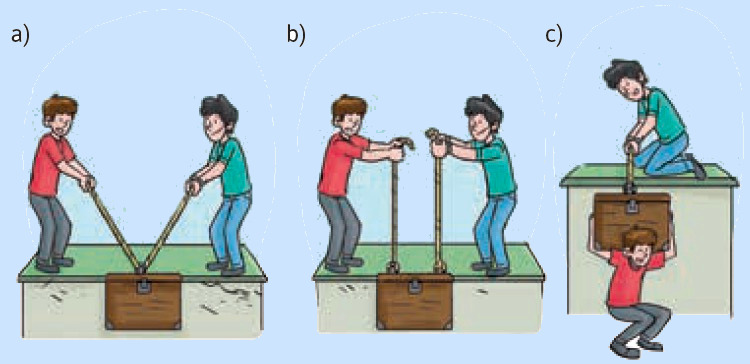
\includegraphics[width=0.8\linewidth]{subir.jpg}
    %\captionof{figure}{Ejemplificación de la magnitud de la energía potencial gravitacional.}
    % \label{fig:gpe}
  \end{figure}%
  Checo y Manolo deben subir un baúl a la azotea de la manera que les implique el menor esfuerzo
  y han imaginado las soluciones que se muestran a continuación.
  Analicen en parejas las propuestas suponiendo que Checo y Manolo tienen la misma fortaleza
  física y respondan.
  \begin{enumerate}
    \item En su opinión, ¿cuál de las soluciones requiere menor esfuerzo de Checo y Manolo?,
          ¿cuál requiere mayor esfuerzo? ¿Por qué?
    \item ¿Creen que algunas de estas soluciones son equivalentes, es decir, que necesitan el
          mismo esfuerzo de Checo y Manolo? ¿Cuáles serían? ¿Por qué?
  \end{enumerate}
\end{boxK}

\subsubsection{Fuerza, magnitud y dirección}
En la lección anterior vimos que una fuerza puede deformar un cuerpo o modificar su estado de
movimiento. Imagina que eres el delantero estrella de tu equipo de futbol y estás por cobrar
el penalti que es la última oportunidad de ganar el partido. Dejando a un lado tu estado de
ánimo, tu aplomo y la habilidad del portero, ¿de qué depende que logres meter el gol?
La respuesta se refiere propiamente a la física involucrada en esta acción: la fuerza.

Si pateas con mucha fuerza, el balón se moverá con gran rapidez y al portero le
resultará más difícil detenerlo o desviarlo; en cambio, si pateas con poca fuerza,
será menor la rapidez con la que salga disparado y el portero podría detenerlo más
fácilmente. Este \emph{tamaño} o intensidad de la fuerza se llama magnitud y se expresa
con una cantidad numérica. Por otro lado, es fácil imaginar la dirección que seguirá
el balón: si lo pateas a la derecha, saldrá disparado a la derecha; si lo pateas
hacia la izquierda, se moverá en esa dirección. ¿Cómo representarías de manera
gráfica estos elementos de la fuerza: magnitud y dirección? A diferencia de otras
cantidades, como la temperatura o la distancia, que se expresan con una cantidad
numérica, la fuerza requiere indicar la magnitud y la dirección, como en el caso
del desplazamiento y la velocidad. Así, la fuerza se representa gráficamente con
una flecha cuya longitud, en una escala adecuada, es proporcional a la magnitud de
la fuerza, y su dirección y su sentido coinciden con la dirección y el sentido de la fuerza.

\subsubsection{Suma de fuerzas}
El concepto de fuerza, como hemos visto, se usa en física para describir la interacción
entre dos cuerpos, pero es común que un cuerpo interactúe con más de uno a la vez;
cuando varias fuerzas actúan sobre un mismo objeto se dice que forman un sistema de fuerzas.

¿Cómo podemos saber el efecto que tendrán varias fuerzas sobre un cuerpo en particular?
Es posible averiguarlo si sumamos las fuerzas considerando sus respectivas magnitudes y
direcciones. En la actividad anterior observaron el cambio del movimiento del aro metálico
al aplicarle distintas fuerzas. ¿En qué dirección y sentido se movió el aro al colocar un
objeto en el vaso? ¿En qué dirección y en qué sentido se aplicó la fuerza? ¿Cómo la representaron?
¿Cómo representaron la fuerza aplicada cuando colocaron dos objetos en el vaso?
¿Qué semejanzas y diferencias observan entre las representaciones anteriores?\\

\begin{minipage}[t]{0.45\textwidth}
  \begin{figure}[H]
    \centering
    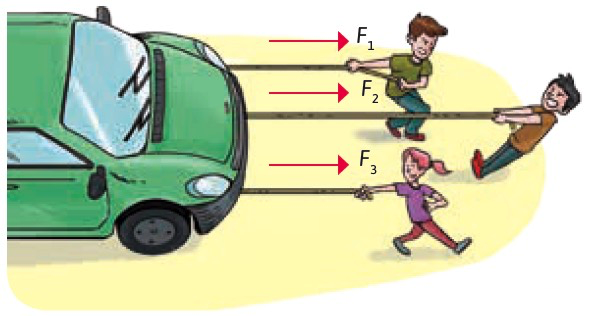
\includegraphics[width=0.8\linewidth]{jalando_carro.jpg}
    \captionof{figure}{Las fuerzas que actúan en la misma dirección y sentido se
      conocen como colineales.}
    \label{fig:jalando_carro}
  \end{figure}
\end{minipage}\hfill
\begin{minipage}[t]{0.45\textwidth}
  \begin{figure}[H]
    \centering
    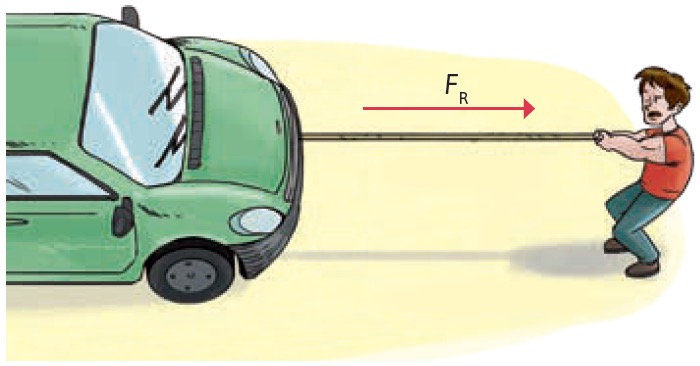
\includegraphics[width=0.8\linewidth]{jalando_carro2.jpg}
    \captionof{figure}{ La fuerza resultante equivale a la suma de todas las
      fuerzas que actúan sobre el objeto.}
    \label{fig:jalando_carro2}
  \end{figure}%
\end{minipage}


Observa la figura \ref{fig:jalando_carro}, donde las tres flechas representan las fuerzas con que
los chicos
jalan el coche; la dirección y el sentido de cada flecha están determinados por la orientación
y el tiro de la cuerda correspondiente, y la longitud de cada flecha muestra la magnitud de la
fuerza aplicada.\\

Si lo piensas un poco, podrás concluir que un hombre de gran fortaleza física, con una cuerda
lo suficientemente resistente, lograría el mismo efecto que los tres chicos juntos, pero aplicando
una sola fuerza; es decir, el efecto de esa única fuerza equivaldría a las tres que aplican los
chicos. ¿Qué longitud y dirección debe tener la flecha que representa la fuerza del hombre fuerte? En el
diagrama de la figura \ref{fig:suma_fuerzas} se representan las fuerzas de los tres chicos. Obsérvala y reflexiona.\\

\begin{figure}[H]
  \centering
  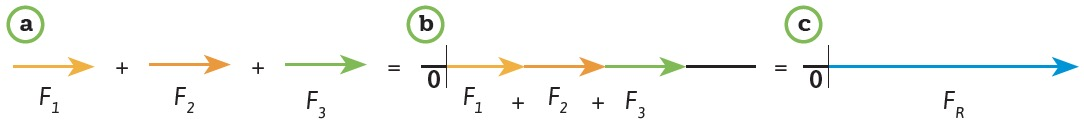
\includegraphics[width=0.9\linewidth]{suma_fuerzas.jpg}
  \captionof{figure}{Suma de fuerzas.}
  \label{fig:suma_fuerzas}
\end{figure}


Como las tres fuerzas actúan en el mismo sentido, las tres tienen la misma dirección y
las tres contribuyen al movimiento del auto, así que la fuerza total aplicada es la suma
de las tres fuerzas (inciso b). Sin embargo, la fuerza del hombre fuerte equivale a la de
los tres chicos, por lo que su magnitud es igual a la suma de las tres anteriores y la
dirección es la misma que la de las fuerzas de los tres chicos. A la fuerza equivalente
a la suma otras fuerzas se le conoce como \textbf{fuerza resultante (FR)}.

Cuando sobre un objeto en reposo actúan dos o más fuerzas en sentidos opuestos,
es posible que el objeto no se mueva. Esto ocurre si se anulan los efectos de las
fuerzas, es decir, si la fuerza resultante es 0 N, o puede ocurrir que el objeto
se mueva de acuerdo con la magnitud y dirección de la fuerza resultante.

\begin{minipage}[t]{0.33\textwidth}
  \begin{figure}[H]
    \centering
    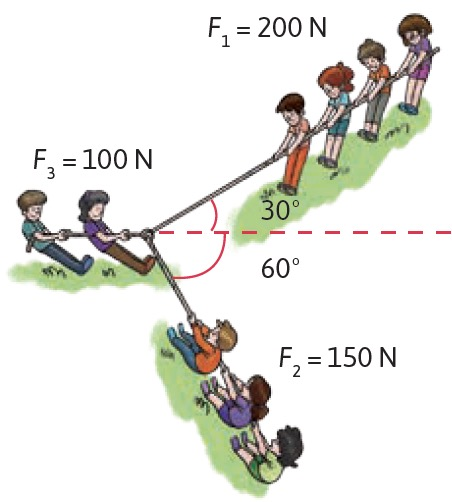
\includegraphics[width=\linewidth]{suma_ninios01.jpg}
    \captionof{figure}{Juego de tirar de una cuerda.}
    \label{fig:suma_ninios01}
  \end{figure}
\end{minipage}\hfill
\begin{minipage}[t]{0.65\textwidth}
  \begin{figure}[H]
    \centering
    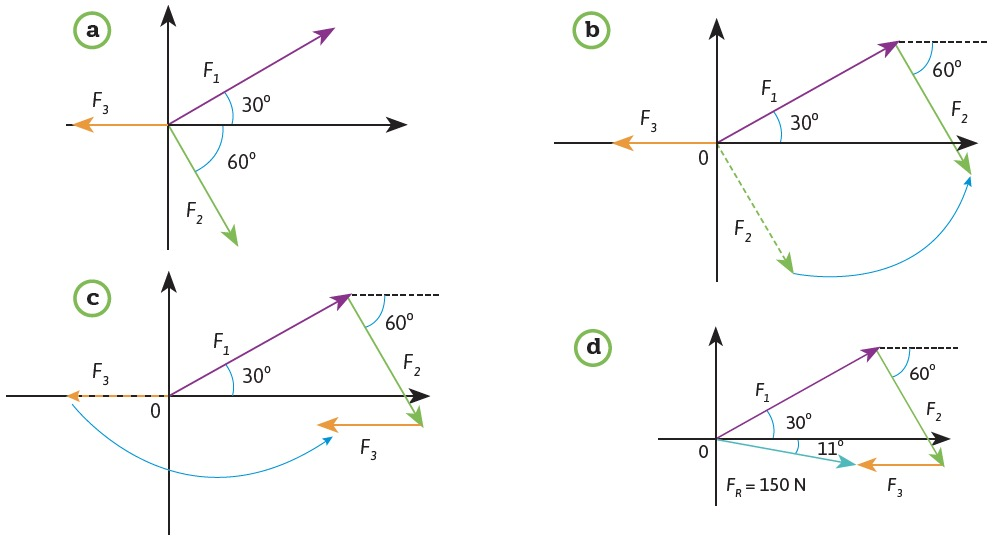
\includegraphics[width=\linewidth]{suma_ninios02.jpg}
    \captionof{figure}{Representación gráfica de las fuerzas y su resultante.}
    \label{fig:suma_ninios02}
  \end{figure}
\end{minipage}\\

Observa la figura \ref{fig:suma_ninios01}. ¿El pañuelo se moverá si cada chico jala con una
fuerza de 50 N?, ¿hacia dónde? Observa que las fuerzas no están orientadas en la misma
dirección y no son precisamente contrarias, pero en este caso también podemos hallar
la suma de las fuerzas mediante un diagrama. Para ello ubicamos nuestro sistema de
fuerzas sobre un plano cartesiano y tomamos la posición inicial del pañuelo como
origen del sistema de referencia. Los ángulos que se muestran se han medido respecto
al eje horizontal.\\

La figura \ref{fig:suma_ninios02} muestra las flechas que representan la fuerza de cada
grupo de niños, la cual se obtiene al sumar las fuerzas que aportan los integrantes
del grupo; esto nos da: 100 N, 150 N y 200 N. Recuerda que todas las flechas se
dibujan con la misma escala, de modo que la longitud de cada una indica la magnitud
de la fuerza que representa.\\

¿Cómo sumamos estas fuerzas? Procederemos de modo similar al caso de las fuerzas
colineales, recordando que las fuerzas no cambian sus efectos si se desplazan
paralelamente, es decir, sin alterar su longitud, dirección y sentido.\\

Dejamos fija la flecha que representa la fuerza $F_1 = 200$ N y desplazamos las
otras dos flechas de manera que una inicie donde termina la anterior,
como muestra la figura \ref{fig:suma_ninios01}. La flecha que va del inicio
de $F_1$ hasta la punta de $F_3$ representa la fuerza resultante, $F_R$.
Dado que esta fuerza no es cero, podemos concluir que el pañuelo se moverá
en la dirección y sentido de la fuerza resultante. Al medir con una regla y
un transportador sobre el diagrama de la figura 1.33d encontramos
aproximadamente que $F_R = 150$ N y forma un ángulo de 11$^\circ$ por debajo
del lado positivo del eje horizontal. Podemos decir que el movimiento del
pañuelo sería el mismo si sólo se aplicara una fuerza de 150 N en un ángulo
de 11$^\circ$ por debajo del sentido positivo del eje horizontal. Este procedimiento
para sumar fuerzas se conoce como método del polígono, por la forma que
se describe al acomodar los vectores.



\newpage
\subsubsection{Ejercicios}
Lee las preguntas y elige los vectores que representan la fuerza necesaria para
equilibrar cada sistema. En las figuras, todos los bloques son iguales
y las poleas tienen masa despreciable (no pesan).
\begin{itemize}
  \item Problema 1
        \begin{boxK}
          \begin{minipage}[t]{0.65\textwidth}
            \footnotesize
            \begin{enumerate}
              \item Supón que los tres chicos que jalan el coche lo hacen con una fuerza
                    de 70 N, 35 N y 52.5 N, respectivamente, y que éstas son las únicas
                    fuerzas que actúan.
                    ¿Cuál es la magnitud de la fuerza resultante?
              \item Observa las imágenes de la derecha y responde.
                    Si cada chico jala con una fuerza de 50 N, todas las fuerzas actúan
                    horizontalmente y no se consideran otras fuerzas, ¿hacia dónde se
                    mueve el pañuelo en cada caso?
              \item Establece un procedimiento para sumar fuerzas que actúan en la misma
                    dirección, ya sea en igual o diferente sentido.
            \end{enumerate}
          \end{minipage}\hfill
          \begin{minipage}[t]{0.3\linewidth}
            \begin{figure}[H]
              \centering
              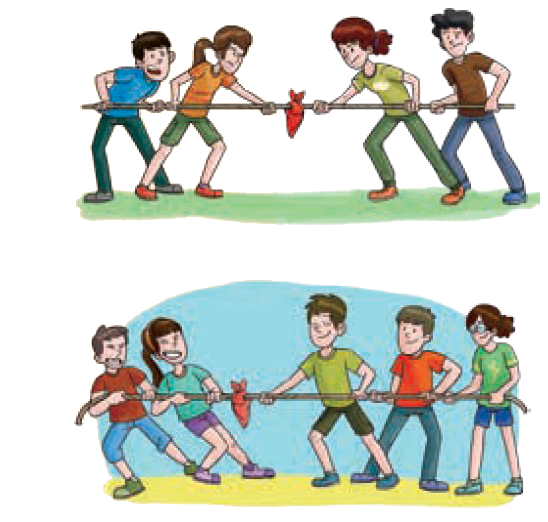
\includegraphics[width=\linewidth]{cuerda_ninios.png}
              % \captionof{figure}{Suma de fuerzas.}
              % \label{fig:suma_fuerzas}
            \end{figure}
          \end{minipage}
        \end{boxK}

  \item Problema 2
        \begin{boxK}
          \begin{figure}[H]
            \centering
            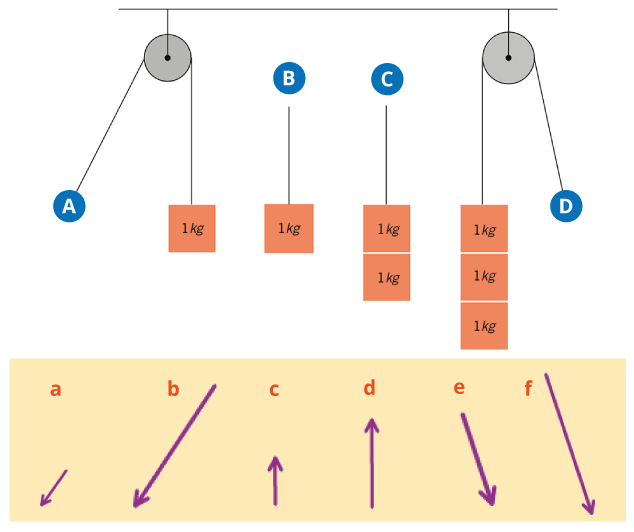
\includegraphics[width=0.6\linewidth]{poleas01.png}
            % \captionof{figure}{Suma de fuerzas.}
            % \label{fig:suma_fuerzas}
          \end{figure}
          \footnotesize
          \begin{enumerate}
            \item ¿Qué vector representa la fuerza necesaria para equilibrar el bloque del
                  sistema A?\\
                  \begin{hoptboxes}
                    \item a \item b \item c \item d \item e \item f
                  \end{hoptboxes}
            \item ¿Qué vector representa la fuerza necesaria para equilibrar el bloque del
                  istema B?\\
                  \begin{hoptboxes}
                    \item a \item b \item c \item d \item e \item f
                  \end{hoptboxes}
            \item ¿Qué vector representa la fuerza necesaria para equilibrar el bloque del
                  sistema C?\\
                  \begin{hoptboxes}
                    \item a \item b \item c \item d \item e \item f
                  \end{hoptboxes}
            \item ¿Qué vector representa la fuerza necesaria para equilibrar el bloque del
                  sistema D?\\
                  \begin{hoptboxes}
                    \item a \item b \item c \item d \item e \item f
                  \end{hoptboxes}
          \end{enumerate}
        \end{boxK}


        \newpage
  \item Problema 3
        \begin{boxK}
          \begin{figure}[H]
            \centering
            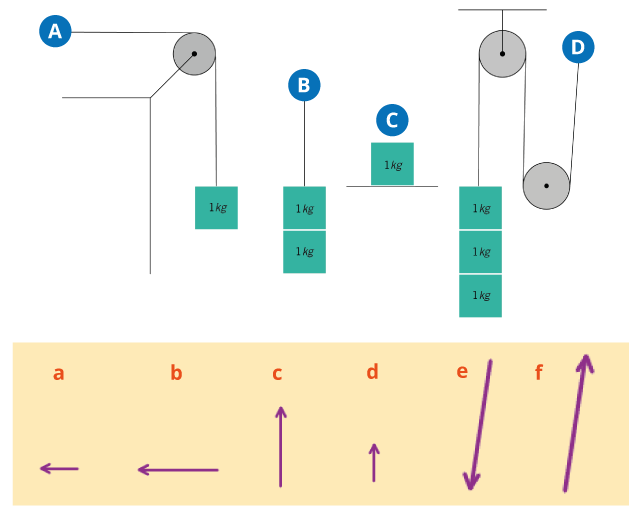
\includegraphics[width=0.9\linewidth]{poleas02.png}
            % \captionof{figure}{Suma de fuerzas.}
            % \label{fig:suma_fuerzas}
          \end{figure}
          \begin{enumerate}
            \item ¿Qué vector representa la fuerza necesaria para equilibrar el bloque
                  del sistema A?\\
                  \begin{hoptboxes}
                    \item a \item b \item c \item d \item e \item f
                  \end{hoptboxes}
            \item ¿Qué vector representa la fuerza necesaria para equilibrar el bloque
                  del sistema B?\\
                  \begin{hoptboxes}
                    \item a \item b \item c \item d \item e \item f
                  \end{hoptboxes}
            \item ¿Qué vector representa la fuerza necesaria para equilibrar el bloque
                  del sistema C?\\
                  \begin{hoptboxes}
                    \item a \item b \item c \item d \item e \item f
                  \end{hoptboxes}
            \item ¿Qué vector representa la fuerza necesaria para equilibrar el bloque
                  del sistema D?\\
                  \begin{hoptboxes}
                    \item a \item b \item c \item d \item e \item f
                  \end{hoptboxes}
          \end{enumerate}
        \end{boxK}
        \newpage
  \item Problema 4
        \begin{boxK}
          \begin{figure}[H]
            \centering
            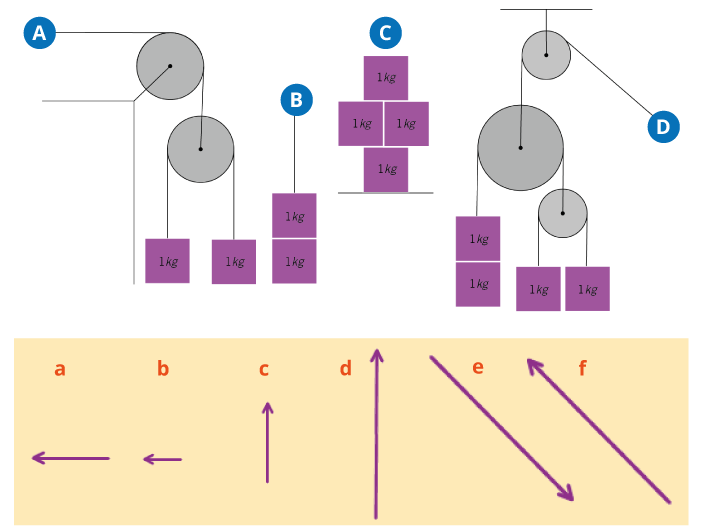
\includegraphics[width=0.9\linewidth]{poleas03.png}
            % \captionof{figure}{Suma de fuerzas.}
            % \label{fig:suma_fuerzas}
          \end{figure}
          \begin{enumerate}
            \item ¿Qué vector representa la fuerza necesaria para equilibrar el bloque del sistema A?\\
                  \begin{hoptboxes}
                    \item a \item b \item c \item d \item e \item f
                  \end{hoptboxes}
            \item ¿Qué vector representa la fuerza necesaria para equilibrar el bloque del sistema B?\\
                  \begin{hoptboxes}
                    \item a \item b \item c \item d \item e \item f
                  \end{hoptboxes}
            \item ¿Qué vector representa la fuerza necesaria para equilibrar el bloque del sistema C?\\
                  \begin{hoptboxes}
                    \item a \item b \item c \item d \item e \item f
                  \end{hoptboxes}
            \item ¿Qué vector representa la fuerza necesaria para equilibrar el bloque del sistema D?\\
                  \begin{hoptboxes}
                    \item a \item b \item c \item d \item e \item f
                  \end{hoptboxes}
          \end{enumerate}
        \end{boxK}
\end{itemize}
\newpage

\subsubsection{Fuerzas en equilibrio}
¿Cómo fue la fuerza resultante que calcularon en el inciso a de la actividad anterior?
Cuando un cuerpo se encuentra en reposo, es decir, sin movimiento, significa que el
resultado de la suma de fuerzas que actúan sobre él es igual a cero: se anulan mutuamente.
Y si usamos el método del polígono para sumarlas podemos ver que la fuerza resultante es
nula; es decir, el inicio de la primera flecha y la punta de la última coinciden en el
mismo punto; cuando esto sucede se dice que las fuerzas están en equilibrio.\\

Más adelante verás que cuando las fuerzas que actúan sobre un objeto están en equilibrio,
pueden ocurrir dos cosas en cuanto al movimiento del objeto: que permanezca en reposo o
que se mueva con velocidad constante.\\

\begin{boxF}
  \begin{center}\bfseries \color{colorrds} Cierre\end{center}

  Volvamos a la situación inicial y supongamos que Checo y Manolo aplican cada uno una
  fuerza de 400 N, y que el baúl pesa 700 N.
  \begin{enumerate}
    \item Si en la primera imagen de la situación de Inicio el ángulo que
          ambas cuerdas hacen con la horizontal es de 45º, ¿es posible que suban el baúl?
    \item ¿Es posible hacerlo según muestran las imágenes b) y c)?
          ¿En cuál se aplica mayor fuerza?
    \item Argumenta tus respuestas a las preguntas de la situación inicial.
  \end{enumerate}

\end{boxF}

\newpage
\subsection{M\'aquinas simples}
\begin{boxK}
  \begin{center}\bfseries \color{colorrds} Inicio\end{center}

  Checo y Manolo aún tienen el problema de subir un baúl a la azotea, y han ideado
  las soluciones que se muestran a continuación. ¿Cuál creen que les implica menor esfuerzo?
  \begin{figure}[H]
    \centering
    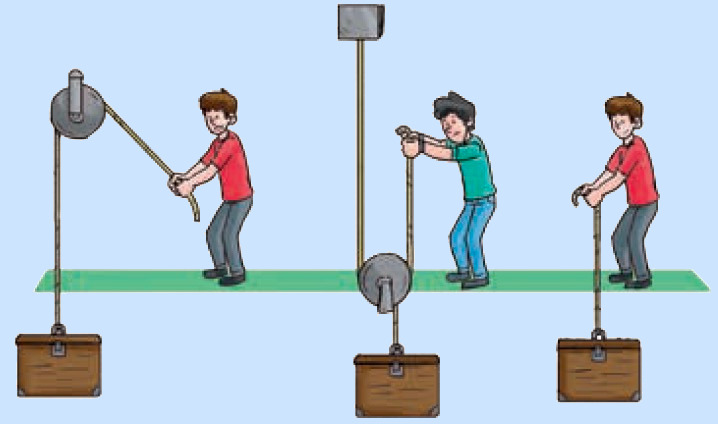
\includegraphics[width=\linewidth]{maq_inicio.jpg}
    % \captionof{figure}{Juego de tirar de una cuerda.}
    % \label{fig:maq_inicio}
  \end{figure}
  \begin{enumerate}
    \item Analiza las propuestas con un compañero y justifiquen sus respuestas.
    \item ¿Consides que son coherentes y lógicas? ¿Cómo podrían comprobar qui\'en
          tiene la respuesta correcta?
  \end{enumerate}
\end{boxK}

La gran pirámide de Keops, en Egipto, es considerada una de las siete maravillas
del mundo antiguo; fue construida alrededor del año 2570 a. n. e., y su base, casi
cuadrada, mide aproximadamente 230 m por lado con una altura original de 146.50 m.
Está construida con bloques de piedra cuyo peso en promedio es de 2500 kg; las
de la base son más grandes y pesadas, cerca de 15 toneladas, y las de la parte
superior pesaban entre 500 kg y 1000 kg. ¿Cómo pudieron los antiguos constructores
transportar, elevar y colocar estas enormes rocas para formar esa colosal obra?\\

Desde la Antigüedad, filósofos, historiadores y constructores especularon
distintas posibles técnicas para el logro de estas impresionantes construcciones,
y en general coinciden en una respuesta: el uso de máquinas simples.\\


Las máquinas simples se clasifican en seis tipos: palancas, ruedas, plano inclinado,
tornos y ruedas, tornillo y cuña. En las siguiente infografía \emph{Maquinas simples}
(figura \ref{fig:SINFI2SB_1E16_U1_S4_b_info})
encontrarás una descripción de ellas.

\subsubsection{La palanca}
Una palanca es una máquina simple que consta de los elementos que muestra la
figura \ref{fig:palanca_gral}.

\begin{figure}[H]
  \centering
  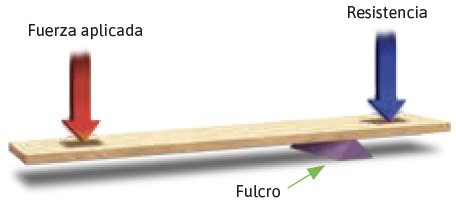
\includegraphics[width=0.6\linewidth]{palanca_gral.jpg}
  \captionof{figure}{Elementos de una palanca.}
  \label{fig:palanca_gral}
\end{figure}

En las palancas se cumple la siguiente relación:

\begin{equation}
  F \times d_F = R \times d_R
\end{equation},

donde $R$ es la resistencia, es decir, la fuerza que se quiere vencer; $F$ es
la fuerza aplicada; $d_F$, la distancia del fulcro (punto de apoyo de la palanca)
al punto de aplicación de la fuerza, y $d_R$, la distancia del fulcro al punto de
aplicación de la resistencia. \\

Las palancas se clasifican en diferentes tipos dependiendo de la ubicación del
fulcro, la resistencia y el punto de aplicación de la fuerza.

\begin{figure}[H]
  \centering
  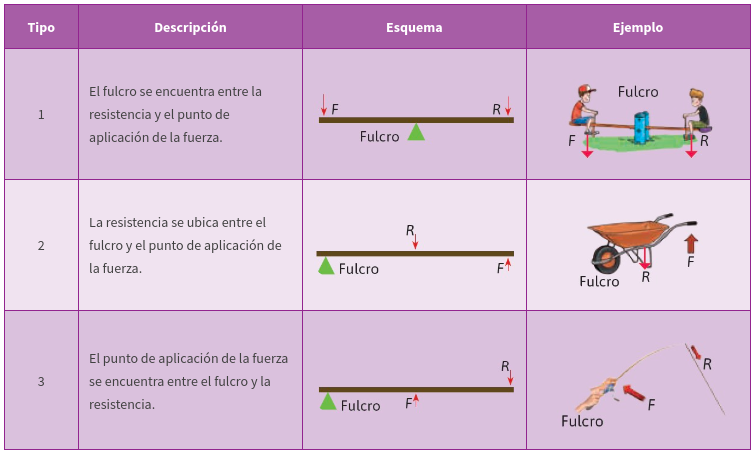
\includegraphics[width=0.9\linewidth]{palanca_clase.jpg}
  \label{fig:palanca_clase}
  \captionof{figure}{Tipos de palancas.}
\end{figure}

En el cuerpo humano también se presentan los tres tipos de palancas, en particular en el sistema locomotor.
\begin{figure}[H]
  \centering
  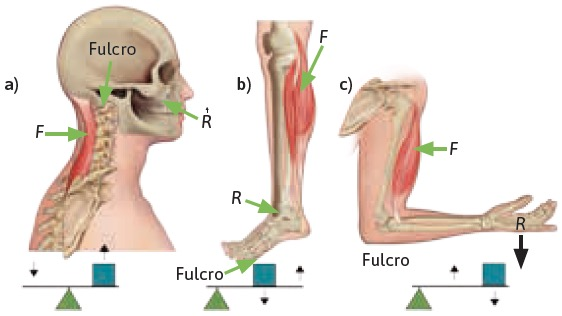
\includegraphics[width=0.6\linewidth]{palanca_body.jpg}
  \captionof{figure}{Elementos de una palanca.}
  \label{fig:palanca_body}
\end{figure}

\subsubsection{Ejercicios}

\begin{boxK}
  \begin{enumerate}
    \item ¿Qué fuerza se debe aplicar a una caja de 100 N de peso para subirla a
          un templete a una altura de 80 cm si se usa una rampa de 240 cm?
    \item Se necesita subir una carga de 500 kg (4900 N) a una altura de 1.5 m
          deslizándola sobre una rampa inclinada, ¿qué longitud debe tener la rampa si
          sólo se puede aplicar una fuerza de 1633.33 N?
    \item ¿Qué relación existe entre el plano inclinado y la cuña?
    \item Analiza la infografía de la figura \ref{fig:SINFI2SB_1E16_U1_S4_b_info} y responde.
          \begin{enumerate}
            \item ¿Qué tareas o trabajos se pueden realizar con máquinas simples?
            \item ¿En qué cambar\'ia el esfuerzo si no se utilizara la máquina simple?
            \item ¿Qué artefactos conoces que combinen máquinas simples?
            \item ¿Cómo funcionan?
          \end{enumerate}
  \end{enumerate}
\end{boxK}

\newpage

\begin{landscape}
  \thispagestyle{empty}
  \begin{figure}[H]
    \centering
    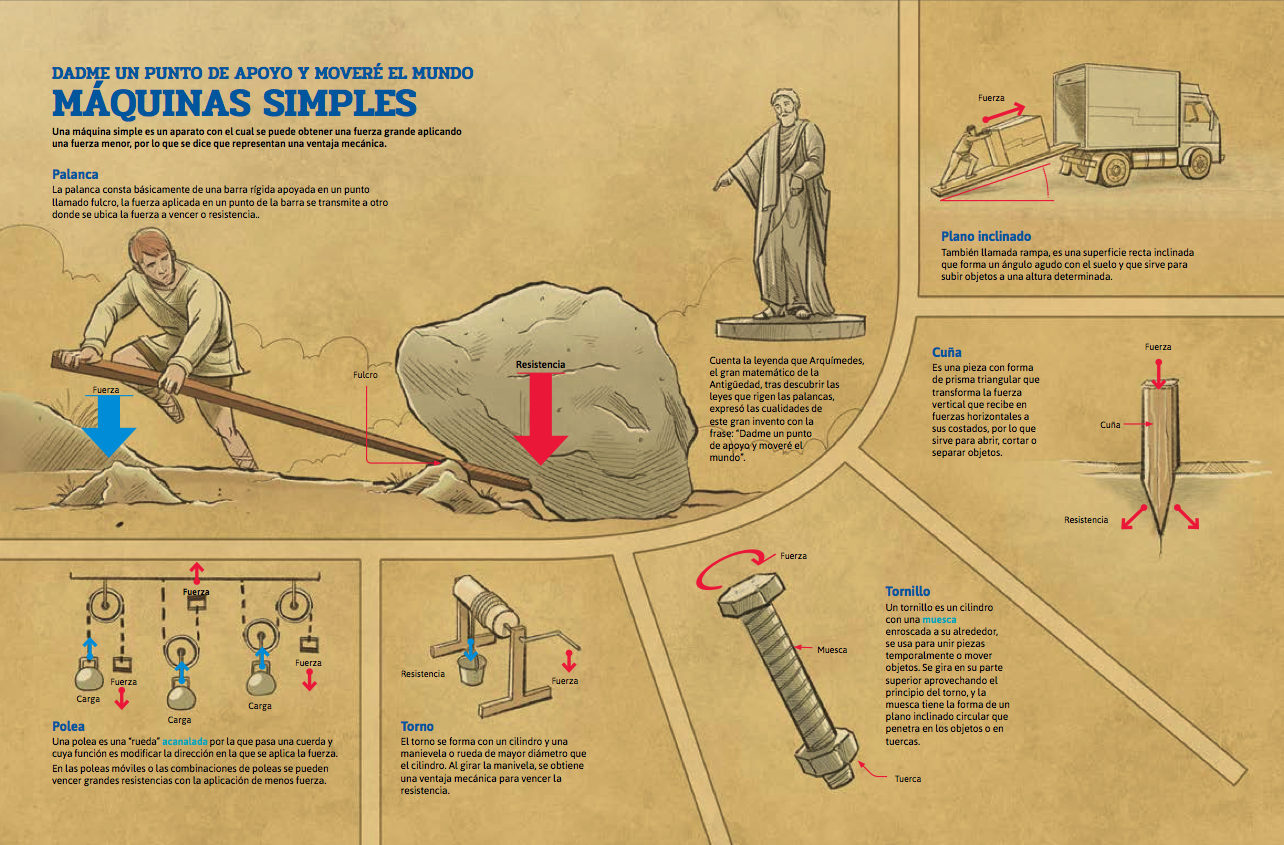
\includegraphics[width=\linewidth]{SINFI2SB_1E16_U1_S4_b_info.png}
    \captionof{figure}{M\'aquinas simples.}
    \label{fig:SINFI2SB_1E16_U1_S4_b_info}
  \end{figure}
\end{landscape}

\newpage

\subsubsection{La rueda y el torno}

La rueda es una máquina simple que utilizas con frecuencia.
¿Qué usos se le dan? La rueda es un objeto circular que gira alrededor de un
eje y sus aplicaciones son muy variadas.\\

\begin{figure}[H]
  \centering
  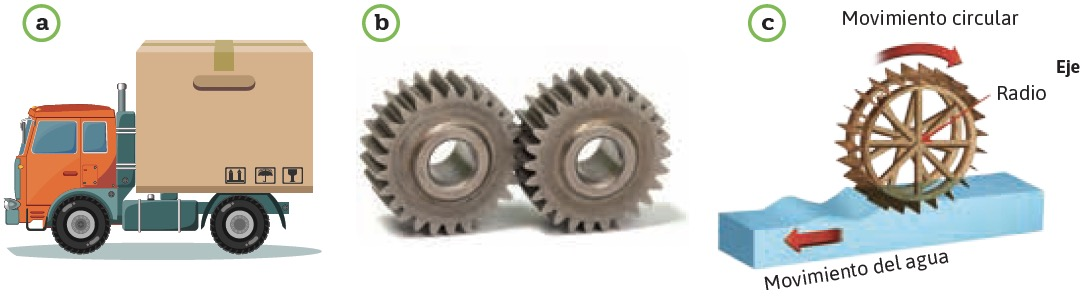
\includegraphics[width=0.9\linewidth]{ruedas01.jpg}
  \captionof{figure}{Tipos de ruedas. a) de transporte, b) engranes, c) de paletas.}
  \label{fig:ruedas01}
\end{figure}

Rueda de transporte: facilita el desplazamiento de objetos y cargas,
ya que gira al contacto con el suelo o las superficies por donde se
mueven los objetos.
Rueda dentada o engrane: se utiliza para transmitir
el movimiento al conectar engranes entre sí.
Rueda de paletas: aprovecha el movimiento en sus extremos para transmitirlo
a su eje como movimiento circular.

El \textbf{torno} es una máquina simple que consiste en un objeto cilíndrico
con dos radios diferentes (uno de ellos puede corresponder al de una manivela).
Al aplicar una fuerza sobre uno de los radios, ésta se transmite al otro de acuerdo
con la siguiente relación:\\

\begin{equation}
  F_1 \times R= F_2 \times r,
\end{equation}
donde $F_1$ es la fuerza aplicada en la parte del cilindro de radio $R$, y $F_2$,
la fuerza que se aplica en la parte del cilindro de radio $r$.

\newpage
\subsubsection{La polea}
La polea es una rueda acanalada por la que pasa una cuerda. En una polea fija simple
se modifica la dirección de una fuerza (figura \ref{fig:poleas_fijas}a); en una polea móvil su eje se
sujeta a la carga y uno de los extremos de la cuerda que la sujeta se amarra a una
superficie fija; la fuerza se aplica en el extremo opuesto (figura \ref{fig:poleas_fijas}b).
Al jalar la cuerda una longitud L, la carga se levantará una longitud ,
y la relación entre las fuerzas cumple la siguiente relación:

\begin{equation}
  F \times L = R \times \left(\frac{L}{2}\right)
\end{equation}

donde $F$ es la fuerza aplicada; $R$, la resistencia, y $L$, la longitud de la cuerda desplazada.

\begin{figure}[H]
  \centering
  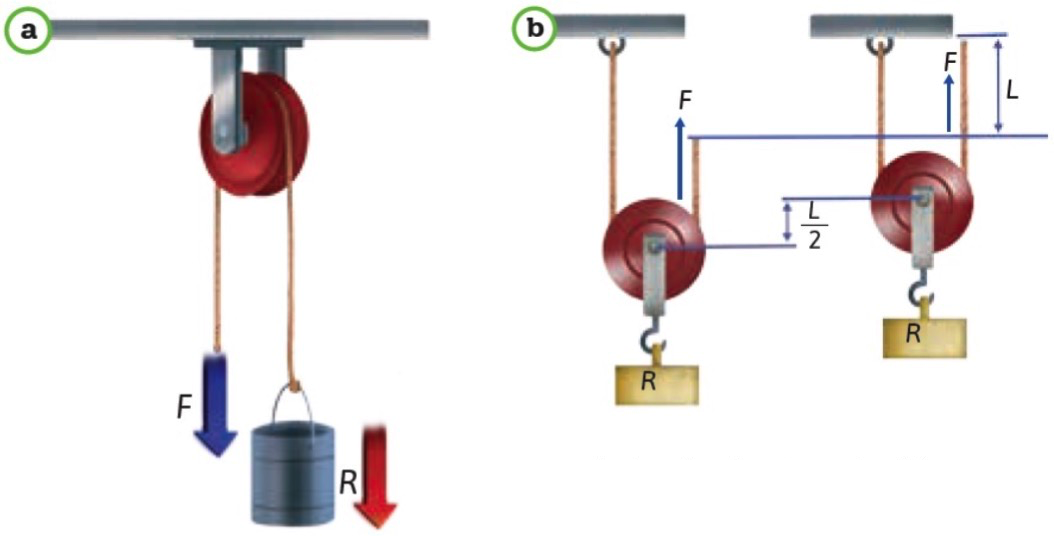
\includegraphics[width=0.9\linewidth]{poleas_fijas.jpg}
  \captionof{figure}{ a. Polea fija, b. polea móvil.}
  \label{fig:poleas_fijas}
\end{figure}


\begin{boxK}
  \begin{center}\bfseries \color{colorrds} Cierre\end{center}
  Retoma la situación de la sección Inicio y responde nuevamente la pregunta.\\
  Se dice que una máquina representa una ventaja mecánica. ¿Qué significa esta frase?
\end{boxK}


\begin{boxH}
  \textbf{Piensa y sé crítico}\\
  ¿Qué tan fuerte puede ser una hoja de papel? En equipo traten que una hoja de
  papel sostenga una libreta. La hoja debe quedar vertical de algún modo y sobre
  ella la libreta; pueden usar un poco de cinta adhesiva o pegamento. Cuando lo hagan,
  preséntelo a sus compañeros, expliquen cómo lo lograron y dibujen un diagrama que
  muestre las fuerzas que actúan sobre la libreta.
\end{boxH}
\newpage
\subsubsection{Ejercicios}
\begin{boxK}
  \begin{enumerate}
    \item Calcula la fuerza que se obtiene en el cilindro de un torno de radio 10 cm si
          sobre la manivela de radio 50 cm conectada al torno se aplica un fuerza de 35 N.
    \item ¿Qué relación existe entre el torno y el tornillo (que es una máquina simple)?
    \item ¿Con qué fuerza se debe jalar un peso de 45 N si se usa una polea fija?, ¿y si
          se usa una polea móvil?
    \item ¿Por qué se utiliza una polea fija si no representa una ventaja en cuanto a la
          aplicación de una fuerza?
    \item Elige las opciones que resuelvan cada problema.
          \begin{enumerate}
            \item ¿Qué fuerza tendrías que aplicar para subir un sillón de 25 N
                  de peso a una altura de 4 m si utilizas un plano inclinado de 5 m?\\
                  \begin{hoptboxes}
                    \item 50 N \item 10 N \item 20 N \item 100 N
                  \end{hoptboxes}
            \item ¿De qué longitud tendrá que ser el plano inclinado por utilizar si deseas
                  subir un peso de 200 N a una altura de 2 m, si tu máxima capacidad te permite
                  aplicar una fuerza de 50 N?\\
                  \begin{hoptboxes}
                    \item 8 m \item  5,000 m \item 0.5 m  \item 80 m
                  \end{hoptboxes}
            \item ¿A qué altura se subió un objeto de 50 N si se aplicó una fuerza de 25 N y
                  se utilizó un plano inclinado de 10 m?\\
                  \begin{hoptboxes}
                    \item 50 m \item  5 m \item 500 m \item 5.5 m
                  \end{hoptboxes}
          \end{enumerate}
  \end{enumerate}
\end{boxK}


\newpage \thispagestyle{plain}
\section{ Leyes de Newton}
\boxabstract{Describe, representa y experimenta
  la fuerza como la interacción entre
  objetos y reconoce distintos tipos de
  fuerza.
  Identifica y describe la presencia de
  fuerzas en interacciones cotidianas
  (fricción, flotación, fuerzas en
  equilibrio).}

\subsection{Primera Ley de Newton}

\begin{boxK}
  \begin{center}\bfseries \color{colorrds} Inicio\end{center}
  En 1977 la sonda espacial Voyager 1 abandonó la Tierra para siempre; su misión original
  era observar de cerca a Júpiter y Saturno, y se estimaba que su aventura duraría sólo
  cuatro años; pero en 2012 la nave alcanzó el borde del Sistema Solar: ahora está más
  lejos que cualquier planeta, a unos 18 mil millones de kilómetros de la Tierra,
  y se espera que siga enviando datos hasta 2025 (cuando agote su batería) mientras
  continúa su viaje por el espacio interestelar.\\

  \begin{wrapfigure}{l}{0.3\textwidth}
    \centering
    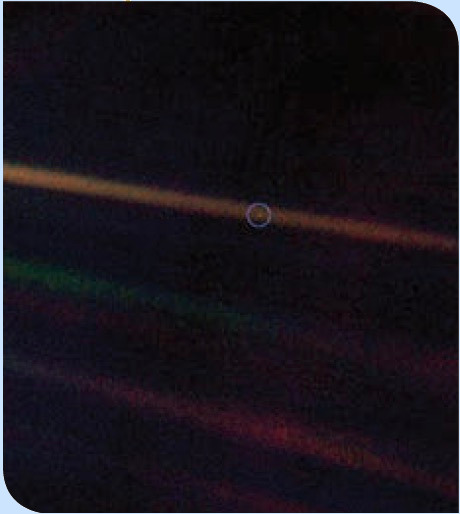
\includegraphics[width=\linewidth]{tierra.jpg}
    \captionof{figure}{Fotografía de la Tierra a 6 400 millones de kilómetros.}
    \label{fig:tierra}
  \end{wrapfigure}

  El 14 de febrero de 1990, cuando se hallaba a 6,400 millones de kilómetros,
  el \textbf{Voyager 1} tomó una foto de la Tierra que la nasa publicó con el
  t\'itulo de \emph{Un punto azul pálido}. El astrónomo Carl Sagan (1934-1996), a propósito de esa foto, escribió:

  \begin{boxF}
    Mira ese punto. Eso es aquí. Eso es nuestro hogar. Eso somos nosotros.
    Ahí ha vivido todo aquel de quien hayas oído hablar alguna vez,
    todos los seres humanos que han existido\dots
    Nuestro planeta es un solitario grano de polvo en la gran penumbra
    cósmica que todo lo envuelve\dots
    En mi opinión, no hay quizá mejor demostración
    de la locura de la soberbia humana que esta distante imagen de nuestro minúsculo
    mundo. Para mí, subraya nuestra responsabilidad de tratarnos los unos a los
    otros más amable y compasivamente, y de preservar y querer ese punto azul pálido,
    el único hogar que jamás hemos conocido.
  \end{boxF}

  Reflexiona y comenta en grupo.

  La batería de la sonda espacial se usa para la telecomunicación, es decir, a la sonda no la impulsa ningún tipo de motor, su combustible se agotó hace mucho tiempo. ¿Por qué entonces se mueve la nave Voyager 1?, ¿continuará así por siempre?
\end{boxK}

\subsubsection{La inercia}
Seguramente has visto el truco en el que un mago quita el mantel de una mesa sobre
el que hay platos, vasos y otros objetos sin que caigan al piso
(figura \ref{fig:inercia}), ¿cómo logra hacerlo? ¿Por qué es importante
usar el cinturón de seguridad al viajar en auto?
¿Por qué un corredor o un automóvil, no pueden frenar de manera inmediata?
¿Sabes qué es la inercia?
\begin{figure}[H]
  \centering
  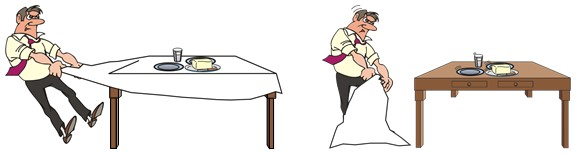
\includegraphics[width=0.6\linewidth]{inercia.jpg}
  \captionof{figure}{Un objeto en reposo tiende a mantenerse en reposo.}
  \label{fig:inercia}
\end{figure}
Cuando abordas un autobús, tanto tú como el vehículo están en reposo. Cuando éste inicia su marcha,
sientes que te mueves hacia la parte trasera como si una fuerza actuara sobre ti en dirección
contraria al movimiento, ¿y cuando el autobús se detiene, te mueves en alguna dirección?
¿Habrá algo en común entre lo que te sucede en el autobús y lo que ocurrió con el huevo que
siguió girando? Existe una tendencia natural de los cuerpos a mantener su estado de movimiento.
Por ello, cuando estás en reposo en un autobús, tu cuerpo tiende a seguir en reposo, y cuando
el vehículo avanza, sientes una fuerza hacia atrás, aunque el autobús vaya hacia adelante;
sin embargo, ésta no es una fuerza real (ningún cuerpo actúa sobre ti): se trata de un efecto
que origina la tendencia de tu cuerpo a permanecer en reposo. Ahora, cuando viajas en un autobús,
la velocidad de tu cuerpo es la misma que la del vehículo, y si éste se detiene, tu cuerpo
sigue un movimiento en línea recta con la misma rapidez que el autobús (figura \ref{fig:autobus}).
Esta tendencia a continuar en reposo o movimiento en línea recta y
a velocidad constante es una propiedad de los cuerpos llamada \textbf{inercia}.

\begin{figure}[H]
  \centering
  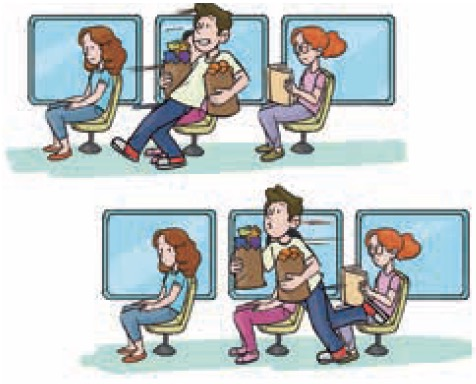
\includegraphics[width=0.4\linewidth]{autobus.jpg}
  \captionof{figure}{Si nos encontramos dentro o sobre un objeto en reposo y
    éste empieza a moverse, sentimos que nos movemos en sentido contrario, pero
    ¿nos movemos o tendemos a permanecer quietos? ¿Y si el objeto está en movimiento
    y se detiene, nos detenemos inmediatamente o seguimos moviéndonos?}
  \label{fig:autobus}
\end{figure}


\begin{figure}[H]
  \centering
  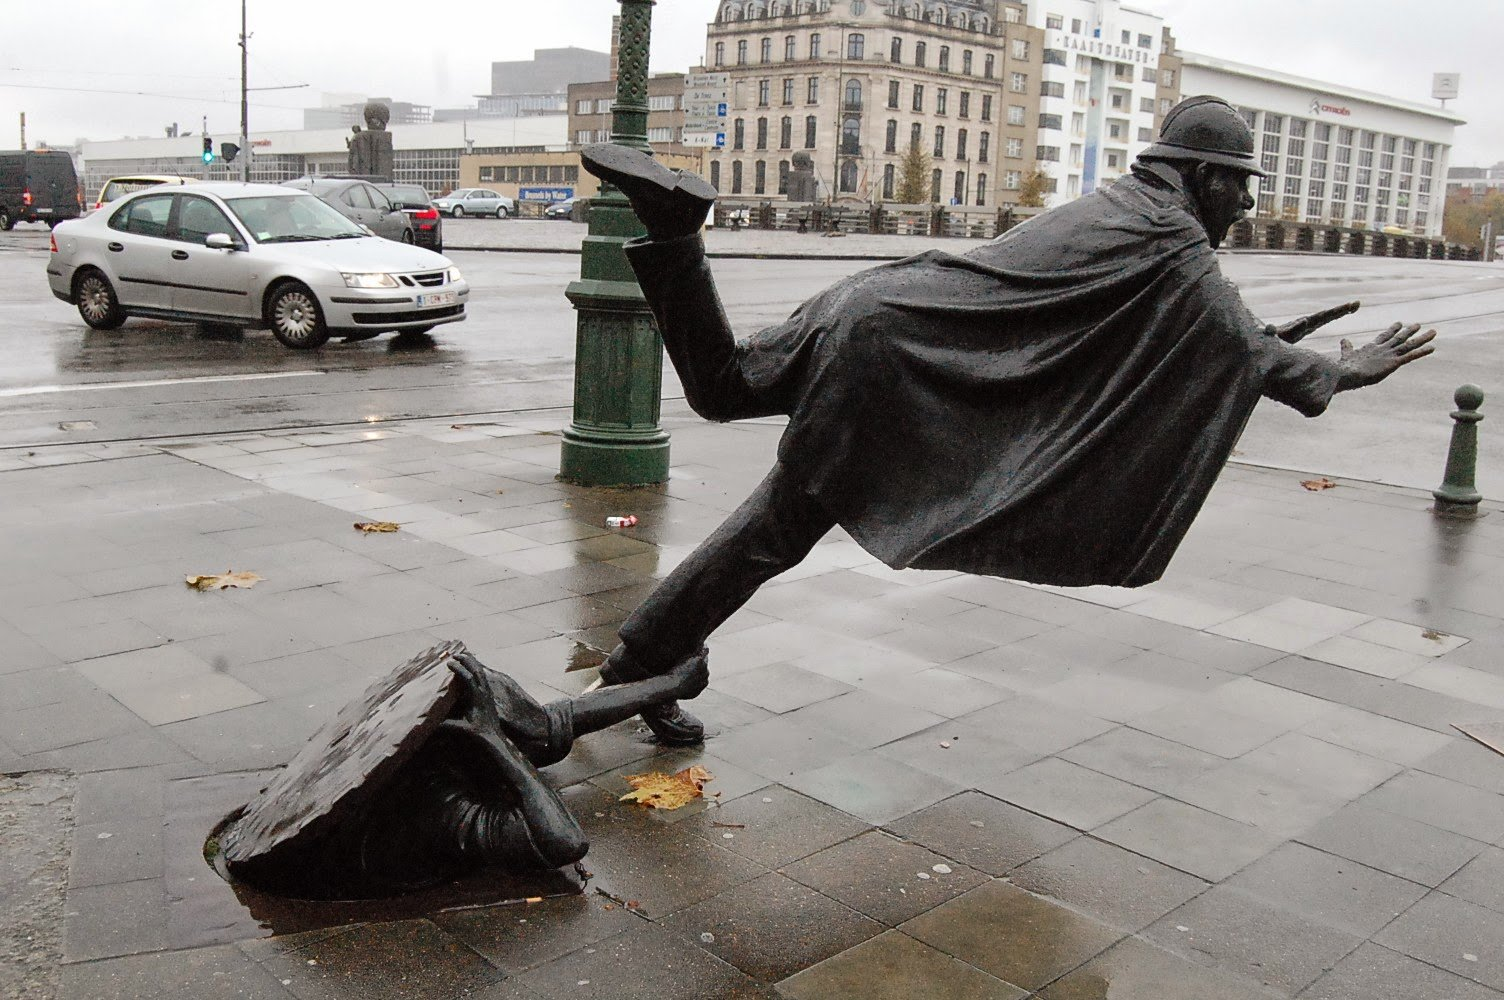
\includegraphics[width=0.4\linewidth]{tropiezo.jpeg}
  \captionof{figure}{Un objeto en movimiento tiende a continuar en movimiento.
    \emph{De Vaartkapoen}, escultura de Tom Franzen, Bélgica.}
  \label{fig:tropiezo}
\end{figure}


\subsubsection{La masa como medida de la inercia}

Existe una relación directamente proporcional entre la masa de los cuerpos y su inercia:
es difícil poner en movimiento los cuerpos con mucha masa, e igualmente es
difícil detenerlos o modificar la dirección de su movimiento; por ello se dice que la masa
es una forma de medir la inercia de los objetos: a mayor masa, mayor inercia; a menor masa,
menor inercia.

\subsubsection{Primera Ley de Newton}

En la Antig\"uedad, Aristóteles afirmaba que el estado natural de movimiento de los
objetos era el reposo y que todos tienden a quedarse quietos. Decía que si un objeto
está en reposo, así se quedará, a menos que se le aplique una fuerza, y si un objeto
está en movimiento, en algún momento se detendrá. Esto nos lo muestra la experiencia, ¿verdad?\\

En nuestra vida cotidiana siempre está presente una fuerza que se manifiesta cuando
dos superficies en contacto se deslizan una sobre la otra y siempre se opone al movimiento:
la fricción. Por eso todos los objetos que se mueven en la Tierra en algún momento se
detienen: si empujas una caja sobre el suelo, no tardará mucho en detenerse; incluso
un auto con ruedas, aunque después de un empujón se mueva una distancia mayor que la
caja, se detendrá, pues la fricción entre la llanta y el eje lo frenará. La fricción
puede ser perjudicial para mecanismos cuyas piezas embonan y se deslizan unas sobre
otras, pues provoca desgaste; para reducir este efecto se usan grasas y lubricantes.
La fricción también está presente en los medios donde hay movimiento; el aire,
el agua y todos los líquidos ofrecen resistencia al movimiento. Pero ¿qué sucedería
con un objeto que se mueve a velocidad constante si no existiera la fricción ni otros
objetos con los que pudiera chocar a su paso? El físico inglés \textbf{Isaac Newton (1642-1727)},
a partir de los estudios de Galileo, respondió esta pregunta con su Primera Ley, que
se enuncia así: Todo objeto tiende a mantener su estado de reposo o movimiento en línea
recta con velocidad constante, a menos que una fuerza que actúe sobre él le obligue a
cambiar ese estado; es decir, un objeto en movimiento conservará su velocidad (rapidez,
dirección y sentido) siempre que sobre él no influya la fricción ni cualquier otra fuerza,
o siempre que las fuerzas que actúan sobre él se anulen mutuamente.

\newpage
\subsubsection{Ejercicios}
\begin{itemize}
  \item Problema 1
        \begin{boxK}
          % \footnotesize
          \begin{minipage}[t]{0.7\linewidth}
            Observa los camiones de la figura \ref{fig:camiones}, responde y argumenta.\\
            \begin{enumerate}
              \item ¿Cuál de ellos será más fácil poner en movimiento?
              \item ¿Cuál podría aumentar más rápido su velocidad?
              \item Si ambos se mueven a la misma velocidad, ¿a cuál le resultaría más difícil frenar?,
                    ¿ambos podrían tomar una curva con la misma facilidad?
              \item Imagina que el camión cargado tira gradualmente parte de su cargamento,
                    y que el conductor pisa el acelerador con la misma fuerza y mantiene el volante en la misma dirección.
                    ¿Qué piensas que pasará con su rapidez?, ¿y si en vez de perder carga fuera recibiendo más?
            \end{enumerate}
          \end{minipage}\hfill
          \begin{minipage}[t]{0.25\linewidth}
            \begin{figure}[H]
              \centering
              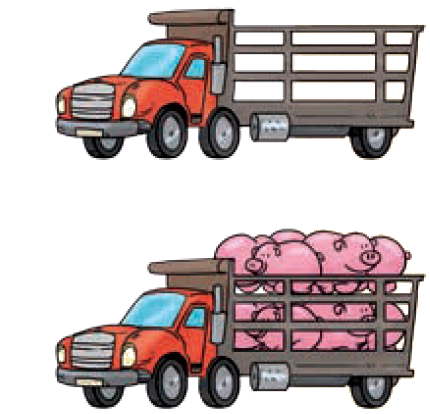
\includegraphics[width=\linewidth]{camiones.png}
              \captionof{figure}{Comparación de dos camiones con diferente masa.}
              \label{fig:camiones}
            \end{figure}
          \end{minipage}
        \end{boxK}
  \item Problema 2
        \begin{boxK}
          \footnotesize
          Elige la respuesta para cada pregunta, a partir de las imágenes de la figura \ref{fig:cerditos}.\\

          \begin{enumerate}
            \begin{minipage}[t]{0.25\linewidth}
              \begin{figure}[H]
                \centering
                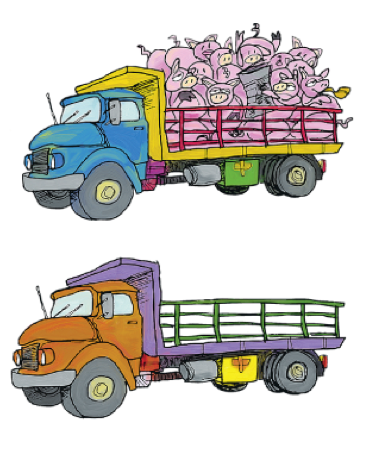
\includegraphics[width=\linewidth]{cerditos.png}
                \captionof{figure}{}
                \label{fig:cerditos}
              \end{figure}
            \end{minipage}\hfill
            \begin{minipage}[t]{0.7\linewidth}
              \item ¿Cuál de ellos será más fácil poner en movimiento?\\

              \begin{hoptboxes}
                \item El camión sin carga. \item El camión cargado.\\
                \item Los dos camiones requieren el mismo esfuerzo.

              \end{hoptboxes}

              \item ¿Cuál podría aumentar más rápido su velocidad?\\

              \begin{hoptboxes}
                \item El camión sin carga.\item El camión cargado.\\
                \item Los dos camiones aumentan su velocidad con la misma rapidez.

              \end{hoptboxes}

              \item Si ambos camiones se movieran a la misma velocidad,
              ¿a cuál de ellos le resultaría más difícil frenar?\\

              \begin{hoptboxes}
                \item El camión sin carga.\item El camión cargado.\\
                \item Los dos camiones requieren el mismo esfuerzo.

              \end{hoptboxes}
            \end{minipage}

            \item  ¿Cuál de los camiones podría tomar una curva con más
                  facilidad si ambos se están moviendo a la misma velocidad?

                  \begin{hoptboxes}
                    \item El camión sin carga.\item El camión cargado.\\
                    \item Los dos camiones requieren el mismo esfuerzo.

                  \end{hoptboxes}

            \item Si el camión cargado va dejando gradualmente parte de su cargamento mientras el
                  conductor pisa el acelerador con la misma fuerza y mantiene el camión en la misma dirección,
                  ¿qué pasa con su rapidez?

                  \begin{hoptboxes}
                    \item La rapidez del cami\'on aumenta.\\
                    \item La rapidez del cami\'on disminuye.\\
                    \item La rapidez del cami\'on no cambia.
                  \end{hoptboxes}

          \end{enumerate}

        \end{boxK}
        \newpage
  \item Problema 3
        \begin{boxK}
          %\footnotesize
          Elige la respuesta para cada pregunta, a partir de las imágenes de la figura \ref{fig:camiones2}.\\

          \begin{enumerate}
            \begin{minipage}[t]{0.25\linewidth}
              \begin{figure}[H]
                \centering
                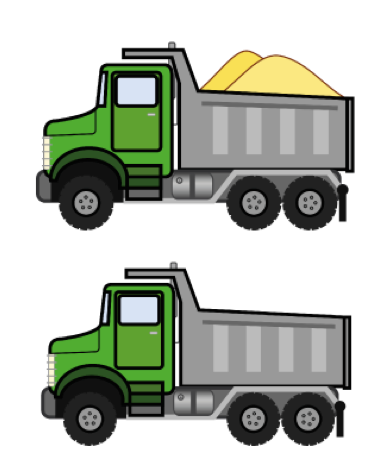
\includegraphics[width=\linewidth]{camiones2.png}
                \captionof{figure}{}
                \label{fig:camiones2}
              \end{figure}
            \end{minipage}\hfill
            \begin{minipage}[t]{0.7\linewidth}
              \item ¿Cuál de ellos será más fácil poner en movimiento?\\

              \begin{hoptboxes}
                \item El camión sin carga.\\
                \item Los dos camiones requieren el mismo esfuerzo.\\
                \item El camión cargado.
              \end{hoptboxes}

              \item ¿Cuál podría aumentar más rápido su velocidad?\\

              \begin{hoptboxes}
                \item El camión sin carga.\\
                \item Los dos camiones aumentan su velocidad con la misma rapidez.\\
                \item El camión cargado.
              \end{hoptboxes}

              \item Si ambos camiones se movieran a la misma velocidad,
              ¿a cuál de ellos le resultaría más difícil frenar?\\

              \begin{hoptboxes}
                \item El camión sin carga.\\
                \item Los dos camiones requieren el mismo esfuerzo.\\
                \item El camión cargado.
              \end{hoptboxes}
            \end{minipage}

            \item  ¿Cuál de los camiones podría tomar una curva con más
                  facilidad si ambos se están moviendo a la misma velocidad?

                  \begin{hoptboxes}
                    \item El camión sin carga.\\
                    \item Los dos camiones requieren el mismo esfuerzo.\\
                    \item El camión cargado.
                  \end{hoptboxes}

            \item Si se reduce la carga de arena de tal manera que la masa
                  del camión sea la mitad de su masa inicial, mientras el conductor pisa el
                  acelerador con la misma fuerza y mantiene el camión en la misma dirección,
                  ¿qué pasa con la acelaración del camión?

                  \begin{hoptboxes}
                    \item Aumenta al doble.\\
                    \item Disminuye a la mitad.\\
                    \item No cambia.
                  \end{hoptboxes}

          \end{enumerate}

        \end{boxK}
        \newpage
  \item Problema 4
        \begin{boxK}
          % \footnotesize
          Elige la respuesta para cada pregunta, a partir de las imágenes de la figura
          \ref{fig:camiones3}.\\

          \begin{enumerate}
            \begin{minipage}[t]{0.25\linewidth}
              \begin{figure}[H]
                \centering
                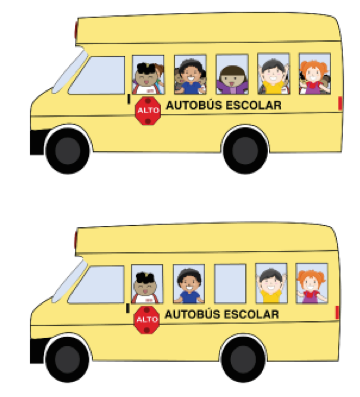
\includegraphics[width=\linewidth]{camiones3.png}
                \captionof{figure}{}
                \label{fig:camiones3}
              \end{figure}
            \end{minipage}\hfill
            \begin{minipage}[t]{0.7\linewidth}
              \item ¿Cuál podría aumentar más rápido su velocidad?\\

              \begin{hoptboxes}
                \item El autobús con más niños.\\
                \item El autobús con menos niños.\\
                \item Los dos autobuses aumentan su velocidad con la misma rapidez.
              \end{hoptboxes}

              \item Si ambos autobuses se mueven a la misma velocidad, ¿a cuál de ellos le resultaría más difícil frenar?\\

              \begin{hoptboxes}
                \item Los dos autobuses requieren el mismo esfuerzo. \\
                \item  El autobús con menos niños. \\
                \item El autobús con más niños.
              \end{hoptboxes}

              \item  Si la masa del segundo autobús es la mitad del primero
              y ambos conductores pisan el acelerador con la misma fuerza y mantienen el autobús en la misma dirección, ¿qué pasa con su aceleración?\\

              \begin{hoptboxes}
                \item Se mantiene igual. \\
                \item Es el doble que la del primero. \\
                \item Es la mitad de la del primero.
              \end{hoptboxes}
            \end{minipage}

            \item  Si el conductor del autobús baja a algunos niños,
                  de tal manera que su masa sea sólo un cuarto de su masa inicial, cuando el conductor pisa el acelerador con la misma fuerza y mantiene el camión en la misma dirección, ¿qué pasa con su acelaración?

                  \begin{hoptboxes}
                    \item Aumenta cuatro veces.\\
                    \item Se mantiene igual.\\
                    \item Disminuye a la cuarta parte.
                  \end{hoptboxes}

            \item El conductor del autobús da vuelta hacia la derecha y los niños
                  sienten una \emph{fuerza} que los empuja. ¿En qué dirección sienten los niños esta fuerza?

                  \begin{hoptboxes}
                    \item Los niños sienten que son empujados hacia abajo. \\
                    \item Los niños sienten que son empujados hacia la derecha del autobús.\\
                    \item Los niños sienten que son empujados hacia la izquierda del autobús.
                  \end{hoptboxes}

          \end{enumerate}

        \end{boxK}
\end{itemize}

\newpage

\begin{boxK}
  \begin{center}\bfseries \color{colorrds} Cierre\end{center}
  Retoma la pregunta de la situación de Inicio y responde.\\
  \begin{enumerate}
    \item ¿Por qué las naves Voyager I y II mantienen su movimiento?
    \item ¿Por qué un mago (o cualquier persona) puede quitar el mantel de
          una mesa con platos, copas y cubiertos sin que ninguno se caiga?
    \item ¿Si cambiaran las condiciones obtendría el mismo resultado;
          por ejemplo, que el mantel fuera de papel de lija o que jalara lentamente
          el mantel, o si en vez de platos y tazas tuviera una caja pesada? ¿Por qué?
    \item ¿Cuándo es benéfica y cuándo es perjudicial la fuerza de fricción?
    \item ¿Por qué un paracaidista puede lanzarse desde muy alto y no sufrir
          daños al llegar a tierra?
  \end{enumerate}
\end{boxK}
\newpage
\subsection{Segunda Ley de Newton}
La segunda ley de Newton, conocida tambien como ley de la aceleración, establece que:
cuando se observa un objeto desde un marco de referencia inercial, la aceleración (a)
del objeto es directamente proporcional a la fuerza neta (En) que actúa sobre él,
y es inversamente proporcional a su masa (m).
La segunda ley de Newton se expresa:
\begin{equation}
  \vec{a}=\frac{\vec{F}}{m}
\end{equation}

La dirección de la aceleración será en la dirección de la fuerza neta que actúa sobre el objeto.

Reordenando la relación masa, aceleración y fuerza queda:
\begin{equation}
  \vec{F}=m\vec{a}
\end{equation}

\subsection{Tercera Ley de Newton}
La tercera ley de Newton o ley de acción y reacción establece que: si dos objetos llamados A y B
interactúan, la fuerza $\vec{F}_{BA}$ ejercida por el objeto A sobre el objeto B es igual en
magnitud y opuesta en dirección a la fuerza $\vec{F}_{AB}$ ejercida por el objeto B sobre el
objeto se puede
expresar:

\begin{equation}
  \vec{F}_{BA}=-\vec{F}_{AB}
\end{equation}


La fuerza que el objeto A aplica sobre el objeto B se conoce como
acción y la fuerza que el objeto B aplica sobre el objeto A se conoce
como reacción. La fuerza de acción tiene la misma magnitud que la
fuerza de reacción, pero en dirección opuesta.

La tercera ley de Newton expresa que las fuerzas siempre se presentan
en pares, es decir, no puede existir una fuerza aislada. Además, estas fuerzas actúan
sobre objetos diferentes, por esta razón no se anulan entre si.

Por ejemplo, la fuerza que la Tierra ejerce sobre la Luna, $\vec{F}_{LT}$, es igual
en magnitud y opuesta en dirección a la fuerza que la Luna ejerce sobre la Tierra, $\vec{F}_{TL}$.
En algunos casos, no es fácil identificar la fuerza de acción y la de reacción.
Por ejemplo, cuando cae una pelota, es la fuerza gravitacional de la Tierra la que ejerce la fuerza
de acción sobre la pelota, por lo tanto, la fuerza de reacción la ejercerá la pelota sobre la Tierra.
Claramente, por su menor masa, es la pelota la que acelera hacia la Tierra, de acuerdo a lo que
establece la segunda ley de Newton. La Tierra también se mueve hacia la pelota pero, por su gran masa,
la aceleración de ésta es despreciable.
\newpage \thispagestyle{plain}
\section{ La aportaci\'on de Newton}
\boxabstract{Analiza la gravitación y su papel en
  la explicación del movimiento de los
  planetas y en la caída de los cuerpos
  (atracción) en la superficie terrestre.}
\subsection{Ley de Gravitaci\'on Universal}
\subsection{Newton, vida y obra, sus aportaciones para la ciencia}
\subsection{El movimiento regular de los cuerpos del Sistema Solar: las leyes de Kepler}
\newpage \thispagestyle{plain}
\chapter{}

\newpage \thispagestyle{plain}
\section{ La energ\'ia y sus manifestaciones}

\begin{center}
  \boxabstract{
    Analiza la energ\'ia mec\'anica (cin\'etica y potencial) y describe casos donde
    se conserva.
  }
\end{center}

\subsection{Tipos de energ\'ia}

Analiza el texto y responde.
?`Conoces la teor\'ia del meteorito que caus\'o la extinci\'on de los dinosaurios
hace 65 millones de años? Los cient\'ificos dicen que cay\'o sobre la pen\'insula
de Yucat\'an y que la energ\'ia del impacto era equivalente a la que liberar\'ian
5,000 millones de bombas at\'omicas como la lanzada sobre Nagasaki. El
meteorito debi\'o tener un di\'ametro mayor a 10 km y moverse a 54,000 km/h.
Debido al impacto se form\'o un cr\'ater de 100 km de di\'ametro, se elev\'o
la temperatura en esa zona y se produjo un enorme resplandor: fragmentos
incandescentes, tanto del meteorito como del terreno donde cay\'o, salieron
disparados provocando incendios en distintas partes del planeta.
Como consecuencia del choque se levant\'o una gran cantidad de polvo
que cubri\'o el cielo e impidi\'o el paso de la luz solar, lo que limit\'o la
fotos\'intesis de las plantas y alter\'o las redes tr\'oficas.
\begin{itemize}
  \item La luz y el calor son manifestaciones de la energ\'ia. ?`Qu\'e piensan que
        provoc\'o la formaci\'on de
        fragmentos incandescentes al caer el meteorito? ?`De
        d\'onde proven\'ia la energ\'ia que caus\'o la luz y el fuego durante el impacto?
  \item Si el meteorito hubiera sido m\'as pequeño, ?`habr\'ia producido tanta
        destrucci\'on? ?`Y si se
        hubiera movido con una rapidez menor?
  \item ?`En qu\'e situaciones de la vida cotidiana han escuchado la palabra
        \emph{energ\'ia}? ?`En esas
        situaciones hay algo que cambie o se transforme? ?`Podr\'ian decir qu\'e es la
        energ\'ia?
\end{itemize}

% \begin{enumerate}
%   \question Es probable que t\'u, tu familia y tus amigos utilicen la palabra \emph{energ\'ia} de
%   manera cotidiana: saben que si la energ\'ia el\'ectrica \emph{se va},
%   la televisi\'on, el refrigerador o la licuadora no funcionan. Es posible
%   que hayan escuchado que en las noticias se refieren a los combustibles f\'osiles
%   como energ\'eticos, y que entre ellos est\'a el petr\'oleo
%   y el gas natural, o que en alg\'un comercial hablen de pilas que \emph{dan m\'as
%   energ\'ia}. Seguramente sabes que si la bater\'ia de un tel\'efono
%   m\'ovil se agota, hay que conectarlos a una toma de corriente el\'ectrica. En tu
%   curso de Ciencias y tecnolog\'ia 1 aprendiste que incluso
%   nosotros necesitamos energ\'ia para realizar nuestras funciones vitales, la cual
%   obtenemos de los alimentos mediante la digesti\'on.

%   Pero, ?`qu\'e es la energ\'ia?, ?`c\'omo se manifiesta? ?`C\'omo se relacionan la energ\'ia
%   y el
%   movimiento, por ejemplo, para que se mueva un autom\'ovil? La energ\'ia tiene
%   manifestaciones muy diversas y es casi seguro que hayas experimentado muchas de
%   ellas.
%   \question Relaciona los tipos de energ\'ia con sus fuentes. En tu cuaderno
%   anota al menos
%   un ejemplo en el que se utilice o aplique cada tipo de energ\'ia.
%   \begin{figure}[H]
%     \centering
%     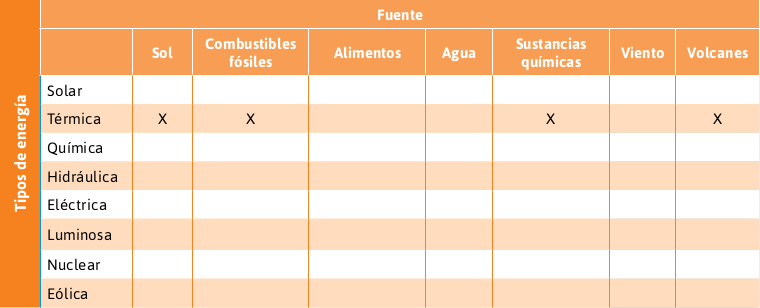
\includegraphics[width=0.8\textwidth]{./Images/tablaS7_tipos_fuentes.png}
%   \end{figure}
%   A partir de tus ejemplos, examina qu\'e usos se dan a la energ\'ia. ?`Qu\'e tienen
%   en
%   com\'un?, ?`en ellos se transforma o modifica algo? Analiza con tus compañeros
%   las respuestas y lo que entienden por energ\'ia; en un texto expresen el
%   significado del t\'ermino.
% \end{enumerate}

\subsubsection{?`Qu\'e es la energ\'ia?}
?`Si la energ\'ia nos parece un concepto tan familiar por qu\'e resulta tan
dif\'icil definirlo? Tal vez porque la energ\'ia es un concepto abstracto: no
es un objeto o una sustancia. A diferencia de la materia, no podemos
ver ni tocar la energ\'ia y, sin embargo, es uno de los conceptos fundamentales
de la ciencia, y quiz\'a el m\'as importante de toda la f\'isica (figura 2.2). Te
sorprender\'a saber que incluso a Isaac Newton se le escap\'o
el concepto de energ\'ia, y que m\'as de un siglo despu\'es de su muerte los
cient\'ificos a\'un cuestionaban su existencia.
Sin embargo, lo que todas las formas de energ\'ia tienen en com\'un es
que pueden transformarse de una forma a otra; por ejemplo, la energ\'ia
el\'ectrica puede provocar movimiento y transformarse en calor que quiz\'a
has percibido al encender una licuadora o un ventilador: las aspas se mueven y
despu\'es de un tiempo el aparato se calienta. Estas transformaciones
pueden cuantificarse, y el n\'umero que resulta es siempre el mismo sin importar
la cantidad de transformaciones que sucedan.
Por ahora definiremos la energ\'ia como la capacidad que tiene una
persona, un objeto, una m\'aquina, un robot, un animal, etc\'etera, para
interactuar con otros objetos. Siempre que hablamos de energ\'ia la relacionamos
con alg\'un cambio, presente o futuro, en los objetos a los que nos
referimos: cambian de estado de movimiento, de forma, de composici\'on (por
ejemplo, durante la combusti\'on), de lugar, etc\'etera.

\subsubsection{La energ\'ia mec\'anica}
?`C\'omo se modifica el estado de reposo o de movimiento de un objeto? En efecto,
con la aplicaci\'on de una fuerza; por tanto, y de acuerdo con la definici\'on
de energ\'ia, existe una estrecha relaci\'on entre la energ\'ia y la fuerza. En todo
cambio de posici\'on o de movimiento de un objeto la energ\'ia est\'a involucrada,
pero para que se d\'e dicho cambio debe tener lugar un desplazamiento.
Si un coche se mueve con cierta rapidez y acelera hasta alcanzar una
rapidez mayor, requerir\'a energ\'ia (la cual proporciona el combustible); el
veh\'iculo, por tanto, est\'a cambiando su estado de movimiento y se realiza
un desplazamiento.
Si una caja inicialmente se encuentra en el piso, cuando se coloca en lo
alto de un librero tiene un cambio en su posici\'on: para subirla se requiri\'o
una cierta energ\'ia y hubo un desplazamiento.
De esta manera, el cambio en el movimiento o en la posici\'on de un objeto
se comprende no s\'olo a partir del concepto de fuerza, sino tambi\'en con base
en el de energ\'ia. La energ\'ia relacionada con el movimiento o la posici\'on de
un objeto se conoce como energ\'ia mec\'anica, y se manifiesta cuando cambia
su estado de movimiento o su posici\'on al aplicarle una determinada fuerza.
Para cuantificar la energ\'ia mec\'anica definiremos dos conceptos nuevos:
energ\'ia cin\'etica y energ\'ia potencial.

\subsubsection{Energ\'ia cin\'etica}
Si has andado en bicicleta, jugado futbol o competido en una carrera, sabr\'as
que despu\'es del ejercicio te sientes cansado. ?`Sab\'ias que Michel Phelps
(1985), nadador estadounidense que ha ganado 28 medallas ol\'impicas, para
entrenar com\'ia lo mismo que cinco adultos? Es un hecho que para llevar a
cabo un esfuerzo f\'isico se requiere energ\'ia, y por eso, despu\'es de
ejercitarnos, sentimos hambre. Con lo anterior queremos decir que el movimiento
est\'a relacionado con la energ\'ia. La energ\'ia que posee un cuerpo debido a
su movimiento se conoce como energ\'ia cin\'etica (del griego kinetos: que se
mueve). Si te has golpeado con un bal\'on de futbol o te has golpeado un dedo
del pie contra un mueble mientras caminas, entonces has sentido los efectos de
la energ\'ia cin\'etica.

Como experimentaste, la energ\'ia cin\'etica de un cuerpo en movimiento depende de
dos variables o magnitudes f\'isicas: su masa (m) y su rapidez (v). La ecuaci\'on
que relaciona ambas variables y define a la energ\'ia cin\'etica ($E_C$) es:

\begin{equation*}
  E_c=\frac{1}{2}mv^2
\end{equation*}

% Las unidades de la energ\'ia cin\'etica, derivadas a partir de su ecuaci\'on, son las
% de masa por las de rapidez al cuadrado: kg m^2/s^2, que corresponden a las
% unidades de la energ\'ia en el SI;es decir, al joule (J). Como sabes, la unidad de fuerza es el
% newton (N), y 1 N equivale a 1 kg m/s$^2$, de manera que:

\( 1 J = 1 kg m^2/s^2 = 1 Nm \)

% \begin{enumerate}
%   \question Considera un carro de la montaña rusa de 300 kg en el que suben
%   ocho
%   personas con una masa promedio de 60 kg. Si en la parte m\'as baja de
%   una curva descendente el carro lleva una rapidez de 120 km/h:
%   \begin{oneparchoices}
%     \items ?`Cu\'al es su energ\'ia cin\'etica en ese instante?
%     \items ?`En qu\'e lugares o situaciones la energ\'ia cin\'etica ser\'a cero?
%     \items ?`C\'omo cambiar\'ia la energ\'ia cin\'etica del carro en la parte m\'as baja
%     de una curva descendente si se suben menos personas?
%   \end{oneparchoices}
%   \question ?`Cu\'al es la masa de un avi\'on que se desplaza a 800 km/h si su
%   energ\'ia cin\'etica es de 30,000,000 J?
%   \question ?`Qui\'en utiliza m\'as energ\'ia, una persona que sube a un edificio de
%   cinco pisos o una que escala a la cima del volc\'an Popocat\'epetl? ?`Por qu\'e?
%   \question ?`Cu\'al tiene mayor energ\'ia, una piedra en reposo en el piso o una
%   con la misma masa que se encuentra a una altura de 5 m tambi\'en en reposo? ?`Por
%   qu\'e?
%   \question ?`Qu\'e objeto producir\'ia mayores cambios al interactuar con otros
%   debido a la atracci\'on gravitacional, uno de menor o uno de mayor masa?
%   \question ?`Un cuerpo puede tener energ\'ia aun sin moverse? Explica.
% \end{enumerate}

\subsubsection{Energ\'ia potencial}
Si colocas un libro en la parte superior de un librero, utilizas una fuerza y
lo desplazas cierta distancia; por tanto, requieres cierta energ\'ia para llevar
a cabo el cambio en su posici\'on, pero el libro, aun inm\'ovil, interact\'ua con la
Tierra (lo que se
manifiesta por su peso), puede caer y desplazarse una distancia. Debido a esta
posibilidad se dice que el libro tiene energ\'ia potencial. As\'i, podemos definir
la energ\'ia
potencial gravitacional como la energ\'ia que tiene un cuerpo en virtud de su
posici\'on
y que est\'a relacionada con la fuerza de gravedad.
\begin{figure}[H]
  \centering
  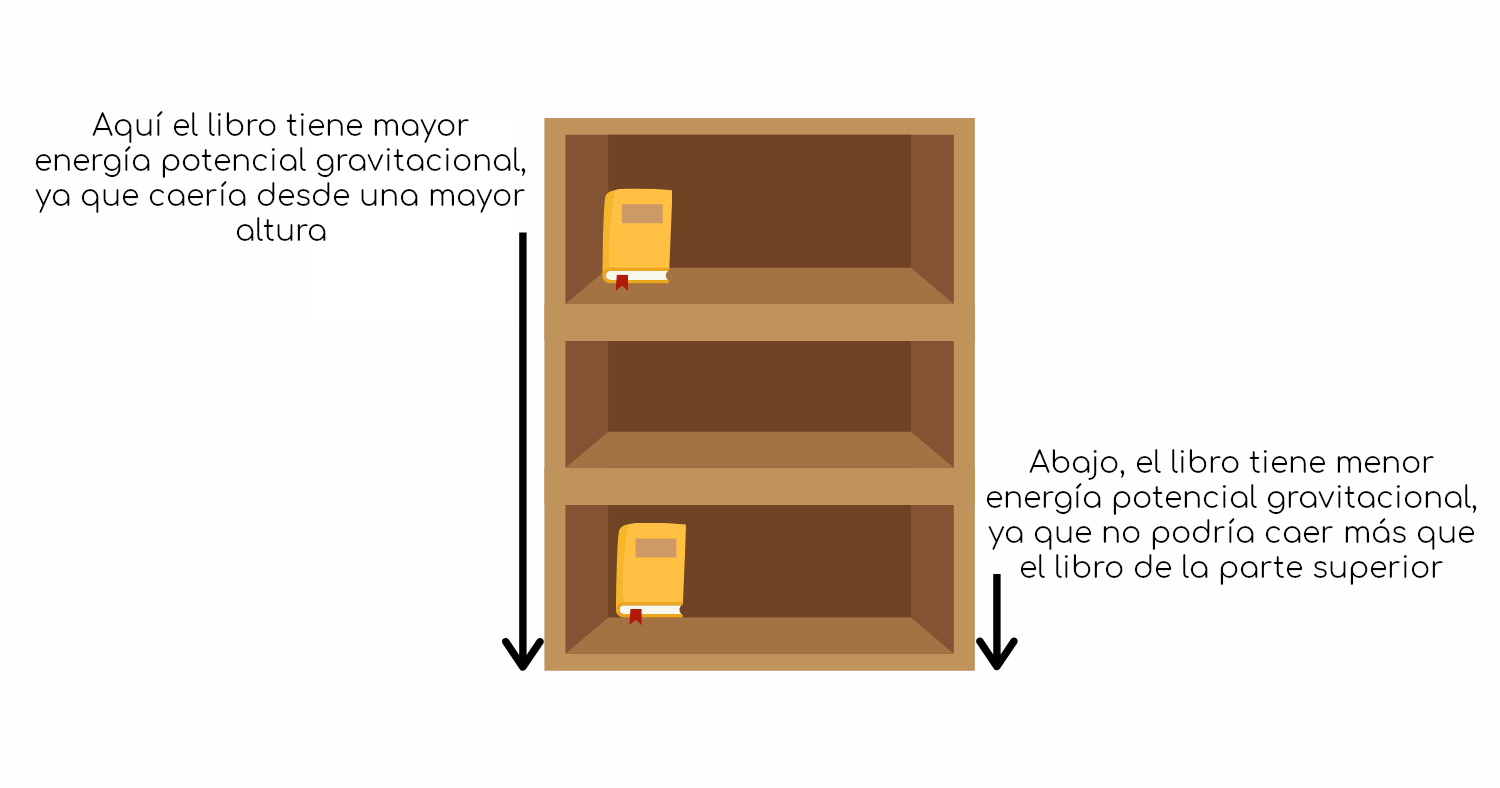
\includegraphics[width=\linewidth]{./Images/Gravitational-potential-energy.png}
  %\captionof{figure}{Ejemplificación de la magnitud de la energía potencial gravitacional.}
  % \label{fig:gpe}
\end{figure}%
La energ\'ia potencial depende de la altura del objeto con respecto a un marco de
referencia, que puede ser la superficie terrestre, la mesa de trabajo, el
pupitre,
de modo que todo objeto que se encuentre en el origen de nuestro marco de
referencia tendr\'a energ\'ia potencial gravitacional igual a cero. Mientras m\'as
alta sea la posici\'on de un objeto en relaci\'on con el origen, mayores ser\'an los
cambios que pueda
producir al interactuar con otros objetos y, por tanto, mayor ser\'a su energ\'ia
potencial
gravitacional.
La energ\'ia potencial tambi\'en depende de la masa de un cuerpo. As\'i, la
ecuaci\'on para el c\'alculo de la energ\'ia potencial gravitacional ($E_P$) involucra
a la masa de un cuerpo (m), la altura a la que se encuentra con respecto al
marco de referencia (h) y la aceleraci\'on de la gravedad (g):
\begin{equation*}
  E_p=mgh
\end{equation*}
La unidad de la energ\'ia potencial, como la de la energ\'ia cin\'etica, es el de un
objeto se relaciona con
su posici\'on.
joule (J). ?`Puedes demostrarlo a partir de la ecuaci\'on?
Antes dijimos que la energ\'ia mec\'anica ($E_m$) de un cuerpo est\'a en funci\'on de su
movimiento y su posici\'on, es decir, la energ\'ia mec\'anica depende de la energ\'ia
cin\'etica y de la energ\'ia potencial de acuerdo con la siguiente expresi\'on:
\begin{equation*}
  E_m=E_c+E_p
\end{equation*}

%\subsubsection{Ejercicios}
% \begin{enumerate}
%   \question ?`Cu\'al es la masa de un objeto que est\'a a una altura de 100 m y cuya
%   energ\'ia potencial es de 1 000 J?
%   \question ?`Puede un objeto en una playa tener la misma energ\'ia potencial
%   gravitacional que otro de la misma masa que est\'a en la Ciudad de M\'exico a una
%   altitud de 2 240 m sobre el nivel del mar? Explica.
%   \question ?`C\'omo es la energ\'ia potencial de un avi\'on de carga que viaja a una
%   altura de 4 000 m a 900 km/h y que tiene una masa de 500 toneladas con respecto
%   a un jet de 250 toneladas que viaja con una rapidez de 1 800 km/h a la misma
%   altura?
%   \question Calcula la cantidad de energ\'ia mec\'anica total de un autom\'ovil que
%   sube una montaña, el cual tiene una masa de una tonelada, se localiza a una
%   altura de 500 m y lleva una rapidez de 50 km/h.


%   Retoma el problema de la situaci\'on de la secci\'on Inicio y verifica si tus
%   respuestas fueron correctas. Despu\'es responde.
%   \begin{enumerate}
%     \item ?`Es posible que un meteorito como el que cay\'o en la pen\'insula de
%     Yucat\'an hace 60 millones de años haya provocado una cat\'astrofe mundial? ?`Por
%     qu\'e?
%     \item ?`Qu\'e tipo de energ\'ia ten\'ia el meteorito? Explica.
%     \item ?`Esa energ\'ia pudo causar la gran cantidad de calor y luz que se supone
%     se gener\'o durante el impacto? ?`Por qu\'e?
%     \item ?`Qu\'e entiendes por energ\'ia?
%   \end{enumerate}
% \end{enumerate}
\subsection{La conservaci\'on de la energ\'ia mec\'anica}

Una actividad muy popular entre algunos j\'ovenes es el skate, donde el skater
se desliza sobre una patineta. Aunque el skate puede practicarse en cualquier
lugar, existen complejos especiales, conocidos como skateparks, equipados
con rampas de varios tipos. El half pipe (medio tubo) es una rampa en forma
de \emph{U} especialmente diseñada para \emph{surfear en seco}.
El skater se desliza desde el borde del half pipe y, haciendo gala de habilidad y equilibro, intenta alguna rutina de trucos que asombren a su p\'ublico:
el skate es un deporte de exhibici\'on, pero, desde otra perspectiva, en \'el hay
mucha f\'isica involucrada.
%\begin{oneparchoices}
%  \item Si el skater se desliza desde el borde del half pipe, sin impulsarse, alcanza el lado opuesto y vuelve, iniciando un movimiento oscilatorio. ?`En qu\'e puntos su energ\'ia potencial alcanza sus valores m\'aximos y m\'inimos?
%  \item Y qu\'e hay de la energ\'ia cin\'etica, ?`en qu\'e puntos alcanza sus valores m\'aximos  y m\'inimos? ?`En qu\'e puntos se logra la mayor rapidez y en cu\'ales la m\'inima?
%  \item Si cuando se lanza el skater s\'olo posee energ\'ia potencial, ?`de d\'onde \emph{sale} su energ\'ia cin\'etica?
%\end{oneparchoices}

\subsubsection{La energ\'ia se transforma}
Hemos hablado mucho acerca de la energ\'ia, pero ?`ya te diste cuenta de que
todav\'ia
no se ha dado una definici\'on precisa y definitiva de lo que es? Ya sabes
bastante sobre
la energ\'ia: que se manifiesta de diversas formas, que existen muchas fuentes y
varios
tipos de energ\'ia e incluso que hay f\'ormulas matem\'aticas para calcularla.
Entonces,
?`qu\'e es la energ\'ia?, ?`cu\'al es su definici\'on? Te asombrar\'a saberlo: actualmente
los f\'isicos contin\'uan sin saber qu\'e es la energ\'ia, y quiz\'a ya no est\'en
interesados en plantear
una definici\'on definitiva. En realidad no importa. Lo que verdaderamente
interesa
saber acerca de la energ\'ia es c\'omo se comporta, c\'omo se transforma.
Veamos c\'omo se comporta, en concreto, la energ\'ia mec\'anica.

%\begin{mybox}{0.60\linewidth}{
%\begin{comfortaa}
%    \color{white} Pr\'actica
%\end{comfortaa}
%  }
%  \begin{enumerate}
%    \question El edificio m\'as alto del mundo hasta el momento- es
%    el Burj Khalifa, ubicado a orillas del golfo P\'ersico en Dubai,
%    ciudad de Emiratos \'arabes Unidos: mide 828 m de altura.
%    Imagina que desde una altura igual a la de la torre se
%    deja caer una pelota de 100 g y considera que no hay
%    fricci\'on del aire ni variaciones en el valor de la aceleraci\'on
%    de la gravedad.
%    \begin{oneparchoices}
%      \items ?`Cu\'anto tiempo tardar\'a la pelota en llegar al suelo?
%      \items ?`Qu\'e velocidad tendr\'a justo antes de tocarlo?
%      \items Calculen en equipo los resultados. Estos problemas no son nuevos
%      para ustedes, pero vamos un poco m\'as all\'a: observar lo que ocurre con la
%      energ\'ia de la pelota.
%      \items Calculen la energ\'ia cin\'etica, potencial y mec\'anica de la pelota
%      cada segundo, desde que se suelta, es decir, desde t = 0 s, y para el valor del
%      tiempo de ca\'ida. Anoten los resultados en una tabla como la siguiente y
%      graf\'iquenlos.
%      \items Aqu\'i presentamos como ejemplo la gr\'afica correspondiente a t = 5 s.
%      Observen que incluimos una gr\'afica circular (figura a) y una de barras (figura
%      b) para optimizar el an\'alisis.
%      \items ?`Cu\'al es el valor de la energ\'ia potencial de la pelota E al
%      momento de soltarla, es decir, en t = 0 s? ?`Cu\'anto vale la energ\'ia cin\'etica?,
%      ?`y la energ\'ia mec\'anica total?
%      \items ?`Qu\'e valor tiene la energ\'ia potencial de la pelota un instante
%      antes de que toque el piso? ?`Cu\'anto vale la energ\'ia cin\'etica?, ?`y la energ\'ia
%      mec\'anica total?
%      \items Ordenen las gr\'aficas seg\'un la secuencia temporal y obs\'ervenlas.
%      ?`Qu\'e notan?, ?`c\'omo cambia la energ\'ia potencial en el transcurso del tiempo?,
%      ?`la cin\'etica?, ?`y la total?
%      \items ?`Qu\'e pasa con la energ\'ia cin\'etica cuando cambia la potencial? ?`Qu\'e
%      relaci\'on hay entre estas cantidades?
%      \items ?`Cu\'ales son sus conclusiones? Reg\'istrenlas en su cuaderno.
%    \end{oneparchoices}
%  \end{enumerate}
%\end{mybox}
Ya conocemos cuatro leyes de la F\'isica. No todas las leyes f\'isicas
se resumen en f\'ormulas matem\'aticas. Ahora consideraremos una ley
relacionada con la energ\'ia; quiz\'a si te pones un poco curioso te
asombre su formulaci\'on porque es un poco distinta de las anteriores.
Richard Feynman (1918-1988), uno de los m\'as ingeniosos, destacados
y extravagantes f\'isicos de la historia y ganador del premio Nobel de
F\'isica en 1965, la explicaba as\'i:
Existe una cierta cantidad, que llamamos energ\'ia, que no cambia
cuando en la naturaleza ocurre un cambio. Es una idea de lo m\'as abstracta
porque es un principio matem\'atico que dice que hay una cantidad que no cambia
cuando algo sucede. No es la descripci\'on de un
mecanismo ni algo concreto. Es tan s\'olo un hecho extraño el que seamos capaces
de calcular un n\'umero, y que al volver a calcularlo despu\'es de observar las
piruetas de la naturaleza, \'este sea el mismo.
\newpage \thispagestyle{plain}
\section{ Los modelos en la ciencia}
\subsection{Explicaci\'on de los fen\'omenos de la naturaleza a partir de modelos}
\subsection{Ideas en la historia entorno a la estructura de la materia}
\subsection{Aspectos b\'asicos del modelo cin\'etico de part\'iculas}
\newpage \thispagestyle{plain}
\section{ Cambios de estado de la materia y el modelo cin\'etico}
\subsection{Propiedades de la materia: forma, volumen, estados de agregaci\'on, compresibilidad, etc\'etera}
\subsection{Cambios de estado de agregaci\'on}

\section{Temperatura y equilibrio t\'ermico}
\subsection{Temperatura}
\subsection{Calor y temperatura}

\newpage \thispagestyle{plain}
\section{ Calor como energ\'ia}
\subsection{Energ\'ia t\'ermica}
\subsection{Calor y otras formas de energ\'ia}
\subsection{Energ\'ia el\'ectrica y medio ambiente}

\newpage \thispagestyle{plain}
\section{ Interacciones el\'ectricas}
\subsection{Fen\'omenos electrost\'aticos}
\newpage \thispagestyle{plain}
\section{ El modelo at\'omico de la materia}
\subsection{Descripci\'on macrosc\'opica y microsc\'opica del Universo}
\subsection{Desarrollo hist\'orico del modelo at\'omico}
\subsection{Caracter\'isticas del \'atomo}
\newpage \thispagestyle{plain}
\chapter{}

\newpage \thispagestyle{plain}
\section{ Corriente el\'ectrica y magnetismo}
\subsection{Corriente el\'ectrica y magnetismo}
\subsection{Electromagnetismo}

\newpage \thispagestyle{plain}
\section{ Electricidad y magnetismo: ondas electromagn\'eticas}
\subsection{Relaci\'on entre electricidad y magnetismo}
\subsection{Inducci\'on electromagn\'etica}
\subsection{Generaci\'on de ondas electromagn\'eticas}
\subsection{La luz visible}
\newpage \thispagestyle{plain}
\section{ Electricidad y temperatura en sistemas biol\'ogicos}
\subsection{La f\'isica del cuerpo humano}
\newpage \thispagestyle{plain}
\section{ Ciencia, tecnolog\'ia y sociedad}
\subsection{Ciencia y tecnolog\'ia aplicada a la salud}
\subsection{Ciencia y tecnolog\'ia en el mundo actual}
\newpage \thispagestyle{plain}
\section{ F\'isica y conocimiento del Universo}
\subsection{La estructura del Universo}
\subsection{?`C\'omo se estudia el Universo?}
\subsection{Los mecanismos de las estrellas}

\newpage \thispagestyle{plain}
\section{ El Sistema Solar}
\subsection{Caracter\'isticas y exploraci\'on del Sistema Solar}
\subsection{Origen del Sistema Solar}

\newpage \thispagestyle{plain}
\section{ Origen y evoluci\'on del Universo}
\subsection{Teor\'ia de la Gran Explosi\'on}

\end{document}